\documentclass[9pt,handout]{beamer}

% beamerthemeFeng.sty
% style file for beamer presentation

% tikz is used to ``draw'' title page and other templates in beamer
\usepackage{tikz,etoolbox}
\usetikzlibrary{shapes,arrows}

\definecolor{UWBlack}{HTML}{000000}
\definecolor{UWWhite}{HTML}{FFFFFF}


\definecolor{UWMathPinkL1}{HTML}{FFBEEF}
\definecolor{UWMathPinkL2}{HTML}{FF63AA}
\definecolor{UWMathPinkL3}{HTML}{DF2498}
\definecolor{UWMathPinkL4}{HTML}{C60078}
\definecolor{UWGrayL1}{HTML}{DFDFDF}
\definecolor{UWGrayL2}{HTML}{A2A2A2}
\definecolor{UWGrayL3}{HTML}{787878}
\definecolor{UWGrayL4}{HTML}{000000}
\definecolor{UWGoldL1}{HTML}{FFFFAA}
\definecolor{UWGoldL2}{HTML}{FFEA3D}
\definecolor{UWGoldL3}{HTML}{FFD54F}
\definecolor{UWGoldL4}{HTML}{E4B429}

\definecolor{carrot}{HTML}{EE693F}
\definecolor{ivory}{HTML}{F1F3CE}
\definecolor{emerald}{HTML}{265C00}
\definecolor{turquise}{HTML}{5BC8AC}
\definecolor{peacockblue}{HTML}{1E656D}
\definecolor{spicy}{HTML}{B51D0A}
\definecolor{bluegreen}{HTML}{5F968E}
\definecolor{rust}{HTML}{9B4F0F}
\definecolor{burntorange}{HTML}{DE7A22}
\definecolor{sea}{HTML}{20948B}
\definecolor{lagoon}{HTML}{6AB187}


% Set colors for different components in a slide
\setbeamercolor{background canvas}{bg=UWWhite}
\setbeamercolor{author}{fg=UWGoldL3}
\setbeamercolor{institute}{fg=UWMathPinkL3}
\setbeamercolor{title}{fg=UWGrayL4}
\setbeamercolor{section in head/foot}{bg=UWBlack, fg=UWGoldL3}
\setbeamercolor{author in head/foot}{fg=UWGoldL3, bg=UWBlack}
\setbeamercolor{title in head/foot}{fg=UWBlack,bg=UWGoldL3}
\setbeamercolor{institute in head/foot}{fg=UWGoldL3, bg=UWBlack}
\setbeamercolor{navigation symbols}{fg=UWBlack}
\setbeamercolor{normal text}{fg=UWGrayL3}
\setbeamercolor{section in toc}{fg=emerald}
\setbeamercolor{subsection in toc}{fg=bluegreen}
\setbeamercolor{frametitle}{fg=UWMathPinkL2, bg=UWGrayL1}
\setbeamercolor{block title}{bg=emerald, fg=ivory}
\setbeamercolor{block body}{bg=peacockblue!20, fg=peacockblue}
\setbeamercolor{section number projected}{bg=turquise,fg=black}
\setbeamercolor{block title example}{fg=rust,
	bg= sea!40}
\setbeamercolor{block body example}{fg= burntorange,
	bg= lagoon!20}

\setbeamerfont{frametitle}{series=\bfseries} % bold frame title
\setbeamerfont{section number projected}{% bold TOC bullet
  family=\rmfamily,series=\bfseries,size=\normalsize}
  
% two common fields in conference presentations
\newcommand\jointwork[1]{\def\insertjointwork{#1}}
\newcommand\conference[1]{\def\insertconference{#1}}

% Title page style
\setbeamertemplate{title page}{
\begin{tikzpicture}[remember picture, overlay]
\fill[UWWhite]
  ([yshift=30pt]current page.west) rectangle (current page.south east);

\fill[UWBlack]
  ([yshift=30pt]current page.west) rectangle (current page.north east);

\node[anchor=east] at ([yshift=-50pt,xshift=-15pt]current page.north east)
  {
  
\includegraphics[width=0.25\linewidth]{./logonitw.png}};

\node[anchor=north west] at ([yshift=-70pt,xshift=15pt]current page.north west) (institute)
	{
	\parbox[t]{.78\paperwidth}{
    \usebeamerfont{institute}\usebeamercolor[fg]{institute}\large\bfseries\insertinstitute}
    };
    
\node[anchor=west] at ([yshift=-45pt,xshift=15pt]current page.north west) (author)
	{
	\parbox[t]{.78\paperwidth}{
    \usebeamerfont{author}\usebeamercolor[fg]{author}\Large\bfseries \insertauthor}
    };


    
\node[anchor=north] at ([yshift=15pt]current page.center) (title)
	{
	\parbox[t]{\textwidth}{\huge\bfseries\centering
	\usebeamerfont{title}\usebeamercolor[fg]{title}\inserttitle}
	};
    
\node[anchor=north] at ([yshift=-40pt]current page.center) (jointwork)
	{
	\parbox[t]{\paperwidth}{\bfseries\centering\insertjointwork}
	};
	
\node[anchor=north] at ([yshift=40pt]current page.south) (jointwork)
	{
	\parbox[t]{\paperwidth}{\centering\insertconference}
	};
\end{tikzpicture}
}

\setbeamertemplate{headline} % add navigation to headline
{%
  \begin{beamercolorbox}{section in head/foot}
    \vskip5pt\bfseries
    \insertnavigation{\paperwidth}
    \vskip2pt
  \end{beamercolorbox}%
}


\renewcommand*{\slideentry}[6]{} % no solid circle in headline

% three-parts footline, color determined in beamer template
\setbeamertemplate{footline}
{
	\leavevmode % vertical mode is ended and horizontal mode is entered. In vertical mode, TeX stacks horizontal boxes vertically, whereas in horizontal mode, they are taken as part of the text line. 
	\begin{beamercolorbox}[wd=.333333\paperwidth,ht=2.5ex,dp=1.125ex,
      leftskip=.3cm,rightskip=.3cm plus1fil]{author in head/foot}
		\usebeamerfont{author in head/foot}\insertshortauthor
    \end{beamercolorbox}%
    \begin{beamercolorbox}[wd=.333333\paperwidth,ht=2.5ex,dp=1.125ex,
      leftskip=.3cm,rightskip=.3cm plus1fil,center]{title in head/foot}
      {\usebeamerfont{title in head/foot}\insertshorttitle}
    \end{beamercolorbox}%
    \begin{beamercolorbox}[wd=.333333\paperwidth,ht=2.5ex,dp=1.125ex,
      leftskip=.3cm,rightskip=.3cm plus1fil]{institute in head/foot}
      \hfill    {\usebeamercolor[fg]{institute in head/foot}\insertshortinstitute}    
	\end{beamercolorbox}%
}

\setbeamertemplate{navigation symbols}{\bfseries\insertframenumber/\inserttotalframenumber}

\setbeamertemplate{sections/subsections in toc}[ball]

% make the itemize bullets pixelated >
\setbeamertemplate{itemize item}{
	\tikz{
		\draw[fill=spicy,draw=none] (0, 0) rectangle(0.075, 0.075);
		\draw[fill=spicy,draw=none] (0.075, 0.075) rectangle(0.15, 0.15);
		\draw[fill=spicy,draw=none] (0, 0.15) rectangle(0.075, 0.225);
	}
}

% make the subitems also pixelated >, but a little smaller and red
\setbeamertemplate{itemize subitem}{
	\tikz{
		\draw[fill=carrot,draw=none] (0, 0) rectangle(0.05, 0.05);
		\draw[fill=carrot,draw=none] (0.05, 0.05) rectangle(0.1, 0.1);
		\draw[fill=carrot,draw=none] (0, 0.1) rectangle(0.05, 0.15);
	}
}

\AtBeginEnvironment{block}{
	\setbeamertemplate{itemize item}{
		\tikz{
			\draw[fill=spicy,draw=none] (0, 0) rectangle(0.075, 0.075);
			\draw[fill=spicy,draw=none] (0.075, 0.075) rectangle(0.15, 0.15);
			\draw[fill=spicy,draw=none] (0, 0.15) rectangle(0.075, 0.225);
		}
	}

	\setbeamertemplate{itemize subitem}{
		\tikz{
			\draw[fill=carrot,draw=none] (0, 0) rectangle(0.05, 0.05);
			\draw[fill=carrot,draw=none] (0.05, 0.05) rectangle(0.1, 0.1);
			\draw[fill=carrot,draw=none] (0, 0.1) rectangle(0.05, 0.15);
		}
	}
}

\setbeamertemplate{blocks}[rounded][shadow=false]

\setbeamercovered{invisible}

\usefonttheme[onlymath]{serif} % change the math font theme

\AtBeginEnvironment{theorem}{%
  \setbeamercolor{block title}{bg=peppercorn, fg=pearl}
  \setbeamercolor{block body}{bg=parsnip, fg=spicy}
}

% set color scheme in different parts 
% please refer to beamer cheatsheet below for details
% http://www.cpt.univ-mrs.fr/~masson/latex/Beamer-appearance-cheat-sheet.pdf

\title[\textbf{}]{Authenticated Key Agreement Scheme With User
 Anonymity and Untraceability for 5G-Enabled
 Softwarized Industrial Cyber-Physical Systems}

\author[\textbf{}]
{Presented to:\\
Prof. Bala Prakasa Rao Killi}

\institute[\textbf{National Institute of Technology, Warangal}]
{Dept. of Computer Science and Engineering\\
National Institute of Technology, Warangal}

\jointwork{Presented by: \\
Mohammed Junaid Anwar 21CSB0B36\\
Ashish Upre 21CSB0B62\\
Ashish Vedula 21CSB0B63}

% use this so appendices' page numbers do not count
\usepackage{appendixnumberbeamer}

\begin{document}

% Title page, navigation suppressed, no page number
{
\beamertemplatenavigationsymbolsempty
\begin{frame}[plain]
\titlepage
\end{frame}
}

% TOC, navigation suppressed, no page number
% {
% \beamertemplatenavigationsymbolsempty
% \defbeamertemplate*{headline}{miniframes theme no subsection no content}
% { \begin{beamercolorbox}{section in head/foot}
%     \vskip\headheight
%   \end{beamercolorbox}}
% \begin{frame}{Outline} 
% \tableofcontents 
% \end{frame} 
% }
% \addtocounter{framenumber}{-2}

% Acknowledgement Section


\begin{frame}{Acknowledgement}

\begin{block}{Gratitude to the Authors}
    We extend our heartfelt gratitude to the authors of the foundational work:
    
    \begin{itemize}
        \item Anil Kumar Sutrala
        \item Mohammad S. Obaidat, Life Fellow, IEEE
        \item Sourav Saha, Student Member, IEEE
        \item Ashok Kumar Das, Senior Member, IEEE
        \item Mamoun Alazab, Senior Member, IEEE
        \item Youngho Park, Member, IEEE
    \end{itemize}
    
    Their pioneering contributions have enabled valuable advancements in secure communication for 5G-enabled industrial cyber-physical systems, addressing critical challenges in information and communication technology.
\end{block}

\end{frame}

% Abstract Section
\section{Abstract}

\subsection{Overview of CPS and Security Challenges}
\begin{frame}{Overview of CPS and Security Challenges}

\begin{block}{Growth and Applications of CPS}
    \begin{itemize}
        \item The rise of Information and Communications Technology (ICT) has expanded the reach of Cyber Physical Systems (CPS).
        \item CPS now impacts fields like:
            \begin{itemize}
                \item Smart grids, smart cities
                \item Transportation, public safety, healthcare
                \item Industrial manufacturing, and more
            \end{itemize}
    \end{itemize}
\end{block}

\begin{block}{Security Concerns}
    \begin{itemize}
        \item \textbf{5G and SDN Integration}: Communication via public channels within industrial CPS (ICPS) through 5G and Software-Defined Networking (SDN).
        \item \textbf{Security Threats}: Increased risk of potential security threats and attacks within ICPS environments.
    \end{itemize}
\end{block}

\end{frame}

% Frame 2: Proposed Solution - UAKA-5GSICPS Scheme
\subsection{Proposed Solution: UAKA-5GSICPS Scheme}
\begin{frame}{Proposed Solution: UAKA-5GSICPS Scheme}

\begin{block}{Objective}
    \begin{itemize}
        \item Introduces the \textbf{UAKA-5GSICPS} scheme, a three-factor user authentication and key agreement protocol.
        \item Specifically designed for 5G-enabled SDN-based ICPS environments.
    \end{itemize}
\end{block}

\begin{block}{Functionality}
    \begin{itemize}
        \item Ensures \textbf{mutual authentication} between authorized users and IoT-based smart devices.
        \item Authentication process is mediated by the SDN controller node for secure real-time data access.
    \end{itemize}
\end{block}

\end{frame}


\section{Introduction}
\subsection{Motivation}

\begin{frame}{Motivation}

\begin{block}{Challenges in Securing ICPS}
    \begin{itemize}
        \item \textbf{Modest Resource Limitations}: Traditional security paradigms are unsuitable for Industrial Cyber-Physical Systems (ICPS), where sensors and actuators operate with limited resources.
        \item \textbf{Heterogeneous Communication}: Ensuring secure communication with session key establishment between diverse, registered users and devices is a significant challenge.
        \item \textbf{Scalability Concerns}: Security measures must avoid becoming bottlenecks as ICPS devices scale up extensively.
    \end{itemize}
\end{block}

\begin{block}{Objective of the Work}
    \begin{itemize}
        \item Proposes an efficient user authentication and session key establishment scheme for secure communication between ICPS users and devices.
    \end{itemize}
\end{block}

\end{frame}
\subsection{Software-Defined/Softwarized Networking}

\begin{frame}{Software-Defined/Softwarized Networking (SDN)}

\begin{block}{Key Concepts of SDN}
    \begin{itemize}
        \item \textbf{Control and Data Plane Separation}:
            \begin{itemize}
                \item Control Plane: Manages control flow and network topology.
                \item Data Plane: Forwards packets based on routes determined by the control plane.
            \end{itemize}
        \item \textbf{Operational Advantages}:
            \begin{itemize}
                \item Efficient error recovery, configuration backup, and operational ease.
                \item Ideal for large-scale deployments.
            \end{itemize}
    \end{itemize}
\end{block}

\begin{block}{Protocols and Implementations}
    \begin{itemize}
        \item \textbf{OpenFlow}: Standard defined by the ONF, facilitating communication between SDN controllers and switches.
        \item \textbf{OVS and OF-CONFIG}: Open vSwitch (OVS) is a popular implementation supporting additional protocols like OF-CONFIG.
        \item \textbf{Industry Adoption}: Companies like Google, Cisco, and IBM use SDN for improved data center efficiency.
    \end{itemize}
\end{block}

\end{frame}

\subsection{5G-Enabled Infrastructure and Its Capabilities}

\begin{frame}{5G-Enabled Infrastructure and Its Capabilities}

\begin{block}{Key Features of 5G}
    \begin{itemize}
        \item \textbf{High-Speed \& Low Latency}:
            \begin{itemize}
                \item Data rate up to 10 Gbps and latency reduce to one-thousandth of a second
            \end{itemize}
        \item \textbf{Advanced Technologies}:
            \begin{itemize}
                \item Small cells, Massive MIMO, mmWave, and Li-Fi, 100 billion device support
            \end{itemize}
    \end{itemize}
\end{block}

\begin{block}{Applications and Use Cases}
    \begin{itemize}
        \item \textbf{Fixed Wireless Access}: Wireless broadband for home internet
        \item \textbf{Industrial IoT \& ICPS}: Smart cities, asset tracking, utilities, agriculture, and more
    \end{itemize}
\end{block}

\begin{block}{Network Slicing}
    \begin{itemize}
        \item Enables creating multiple virtual networks from one physical network.
        \item Supported by technologies like NFV, MEC, and SDN for managing high-traffic environments.
    \end{itemize}
\end{block}

\end{frame}
\subsection{Network Model of UAKA-5GSICPS}

\begin{frame}{Network Model of UAKA-5GSICPS}

\begin{block}{Components}
    \begin{itemize}
        \item \textbf{Smart Devices}: n\(_{sd}\) IoT-enabled smart devices \{SD\(_j\) \mid j = 1, 2, 3,..., n\(_{sd}\)\} connected to the data plane switches.
        \item \textbf{Data Plane}: Switches responsible for forwarding data packets to connected devices.
        \item \textbf{Control Plane}: n\(_{cn}\) controller nodes \{CN\(_i\) \mid i = 1, 2, 3,..., n\(_{cn}\)\} manage network topology and user authentication.
    \end{itemize}
\end{block}

\begin{block}{Authentication Process}
    \begin{itemize}
        \item Controller nodes authenticate registered users U\(_k\) for secure session establishment with smart devices.
    \end{itemize}
\end{block}

\begin{block}{Interfaces}
    \begin{itemize}
        \item \textbf{Northbound Interface}: Connects control plane to higher-level entities (users).
        \item \textbf{Southbound Interface}: Connects data plane to lower-level entities (smart devices/access points).
    \end{itemize}
\end{block}

\end{frame}

\begin{frame}{Network Model}

\begin{block}{5G-Enabled Softwarized ICPS}
    \centering
    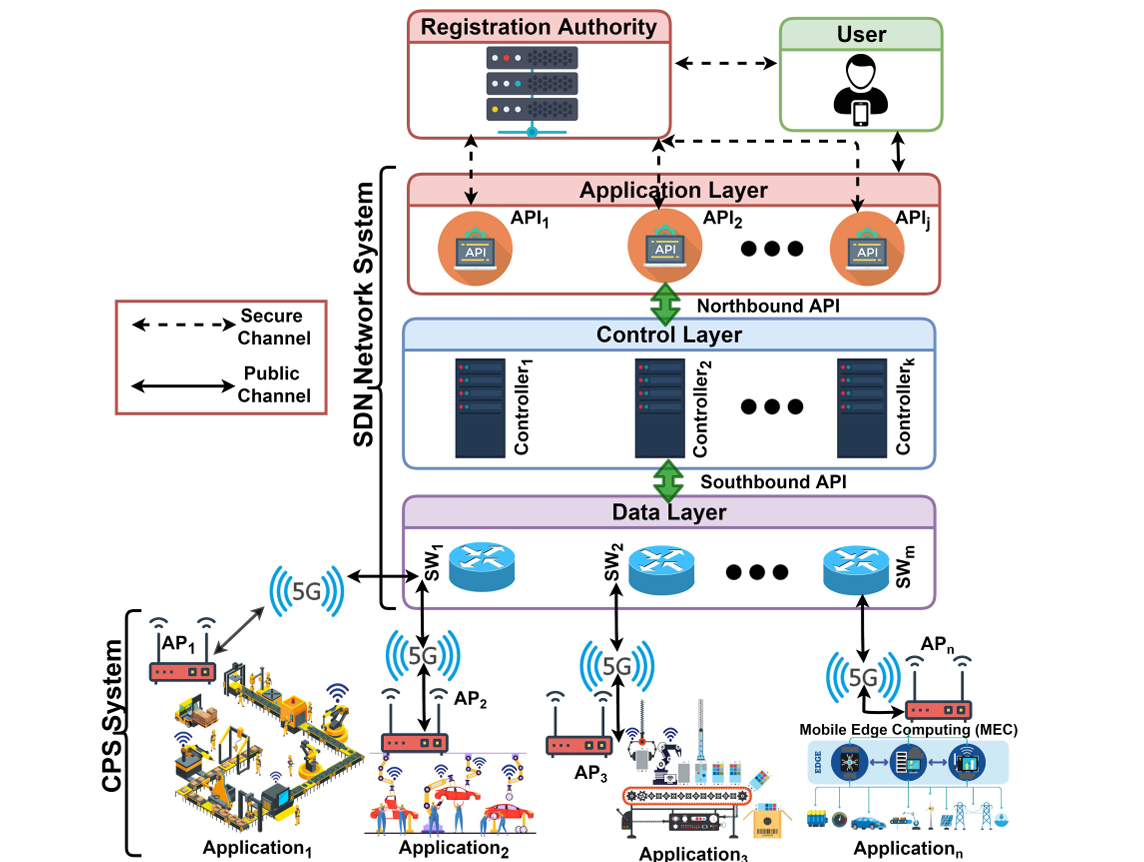
\includegraphics[width=0.8\textwidth]{model.png} % Adjust width as needed
    \caption{\\Network Model of the proposed scheme.}
\end{block}

\end{frame}
\subsection{Attack Model}

\begin{frame}{Attack Model}

\begin{block}{Communication Vulnerabilities}
    \begin{itemize}
        \item Communication between smart devices and users typically occurs via insecure channels. So, An adversary $\mathcal{A}$ can compromise data shared between them.
    \end{itemize}
\end{block}

\begin{block}{Threat Models}
    \begin{itemize}
        \item \textbf{Dolev-Yao Threat Model (DY Model)}:
        \begin{itemize}
            \item $\mathcal{A}$ can eavesdrop, modify, delete, and inject fake information.
        \end{itemize}

        \item \textbf{Canetti-Krawczyk Model (CK-Adversary Model)}:
        \begin{itemize}
            \item $\mathcal{A}$ can hijack sessions and compromise session states, keys, and short-term secrets.
        \end{itemize}
    \end{itemize}
\end{block}

\begin{block}{Security Considerations}
    \begin{itemize}
        \item Session keys must be constructed from both short-term and long-term secrets to prevent Ephemeral Secret Leakage (ESL) attacks.
        \item The Registration Authority (RA) is considered a fully trusted entity in the ICPS environment.
    \end{itemize}
\end{block}

\end{frame}

\subsection{Research Contributions}

\begin{frame}{Research Contributions}

\begin{itemize}
    \item \textbf{Design of UAKA-5GSICPS}: A new three-factor user authentication and key agreement scheme specifically for SDN-based ICPS.
    \item \textbf{Security Analysis}: The scheme is analyzed against various known attacks, proving its security.
    \item \textbf{Formal Security Verification}: Utilizes the AVISPA tool to demonstrate resilience against replay and man-in-the-middle attacks.
    \item \textbf{Comparative Analysis}: Detailed comparison with existing schemes shows:
    \begin{itemize}
        \item Comparable communication and computation overhead.
        \item Enhanced security features.
        \item Practical implementation potential in real-world applications.
    \end{itemize}
    
\end{itemize}

\end{frame}
\section{Related Works}
\begin{frame}
\subsection{Introduction}
\frametitle{Related Works}

\begin{itemize}
    \item In 2015, NIST published an overview on the security of industrial control systems \cite{NIST2015}.
    \item In 2017, Molina et al. addressed cyber security in SDN for ICPS, focusing on access control \cite{Molina2018}.
    \item Taylor et al. and Chong et al. discussed security challenges in connecting IT with CPS devices \cite{Taylor2017, Chong2019}.
\end{itemize}

\end{frame}
\subsection{Key Contributions and Limitations}
\begin{frame}

\frametitle{Key Contributions and Limitations}

\begin{itemize}
    \item Chen et al. proposed an efficient user authentication scheme but it suffers from privileged insider attack \cite{Chen2017}.
    \item Harishma et al. introduced a key agreement scheme for heterogeneous CPS, but it is vulnerable to ESL attacks \cite{Harishma2018}.
    \item Eldefrawy et al. proposed an authentication protocol for industrial IoT, but it lacks mutual authentication \cite{Eldefrawy2019}.
    \item Renuka et al. offered a secure password-based authentication scheme for M2M networks, yet its adoption remains limited \cite{Renuka2019}.
\end{itemize}

\end{frame}
\subsection{Summary and Proposed Contribution}
\begin{frame}
\frametitle{Summary and Proposed Contribution}

\begin{itemize}
    \item Many existing schemes are vulnerable or impractical for real-world applications.
    \item Proposed: A novel user authentication scheme for ICPS that:
    \begin{itemize}
        \item Provides full anonymity and untraceability.
        \item Is secure against modern attack strategies.
        \item Supports user credentials update and dynamic IoT device addition.
    \end{itemize}
    \item Viable for real-time ICPS applications with competitive computational and communication costs.
\end{itemize}

\end{frame}




\section{Proposed Scheme}
\subsection{Introduction to proposed method}
\begin{frame}
    \frametitle{Introduction to UAKA-5GSICPS}
    \begin{itemize}
        \item \textbf{Overview}: The proposed scheme, UAKA-5GSICPS addresses the growing security concerns in modern industrial systems.
        
        \item \textbf{Key Phases}:
        \begin{itemize}
            \item System Bootstrap Phase: Initializes the system components.
            \item Pre-deployment Phase: Prepares controller nodes and IoT smart devices for integration.
            \item User Registration Phase: Allows users to register securely within the system.
            \item Login Phase: Facilitates user access through secure login procedures.
            \item Authentication and Key Agreement Phase: Establishes trust and secure communication between users and devices.
            \item User Credentials Update Phase: Enables users to update their credentials as needed.
            \item Dynamic Smart Device Addition Phase: Allows for the seamless integration of new IoT devices into the existing system.
        \end{itemize}

        \item \textbf{Assumptions}:
        \begin{itemize}
            \item Trusted entities: The Registration Authority (RA) and controller nodes are considered trusted.
            \item Synchronized Clocks: All entities maintain synchronized clocks to prevent replay attacks.
        \end{itemize}
    \end{itemize}
\end{frame}
\subsection{A. System Bootstrap Phase}
\begin{frame}
    \frametitle{A. System Bootstrap Phase}
    \textbf{Overview:} The System Bootstrap Phase is conducted by the Registration Authority (RA) to initialize system parameters for secure communication. Key steps include:

    \begin{enumerate}
        \item \textbf{Parameter Selection}:
        \begin{itemize}
            \item The RA selects a large prime number \( p \).
            \item Defines a non-singular elliptic curve \( E_p(a, b) \): \( y^2 = x^3 + ax + b \, (\text{mod} \, p) \) over a Galois Field \( GF(p) \) or Finite Field  \( \text{z}_{p} \) .
            \item Specifies a base point \( P \) on \( E_p(a, b) \) with order approximately \( p \) and includes a point at infinity \( O \).
            \item Chooses a collision-resistant one-way hash function \( h(\cdot) \).
        \end{itemize}
        
        \item \textbf{Private and Public Key Generation}:
        \begin{itemize}
            \item The RA selects a private key \( \text{pr}_{RA} \in Z^*_p \).
            \item The corresponding public key \( \text{Pub}_{RA} \) is computed as \( \text{Pub}_{RA} = \text{pr}_{RA} \cdot P \).
            \item The private key \( \text{pr}_{RA} \) is kept secret, while \( \text{Pub}_{RA} \) and \( h(\cdot) \) are made publicly available.
        \end{itemize}
    \end{enumerate}

    \textbf{Purpose:} These steps ensure the secure initialization of parameters necessary for the authentication and key agreement processes in UAKA-5GSICPS.
\end{frame}
\subsection{B. Pre-Deployment Phase}
\begin{frame}
    \frametitle{B. Pre-Deployment Phase}
    \textbf{1. Controller Nodes Enrollment\\}
    \textbf{Objective:} Enroll controller nodes \(\text{CN}_i\) with secure identities and credentials.

    \textbf{Steps for Controller Nodes Enrollment}
    \begin{enumerate}
        \item \textbf{Generate Pseudo-Identity}:
        \begin{itemize}
            \item RA computes \( \text{RID}_{\text{CN}_i} = h(\text{ID}_{\text{CN}_i} || \text{pr}_{\text{RA}}) \).
            \item Picks private key \( \text{pr}_{\text{CN}_i} \in Z^*_p \) and calculates public key \( \text{Pub}_{\text{CN}_i} = \text{pr}_{\text{CN}_i} \cdot P \).
        \end{itemize}
        \item \textbf{Random Secret and Certificate Generation}:
        \begin{itemize}
            \item Selects random secret \( r_{\text{CN}_i} \in Z^*_p \), computes \( R_{\text{CN}_i} = r_{\text{CN}_i} \cdot P \).
            \item Generates certificate \( \text{Cert}_{\text{CN}_i} = \text{pr}_{\text{RA}} + h(\text{RID}_{\text{CN}_i} || \text{Pub}_{\text{RA}} || \text{Pub}_{\text{CN}_i}) \cdot r_{\text{CN}_i} \;(\text{mod} \; p) \).
        \end{itemize}
        \item \textbf{Preload and Secure Deletion}:
        \begin{itemize}
            \item RA stores \( \{\text{RID}_{\text{CN}_i}, \text{pr}_{\text{CN}_i}, \text{Pub}_{\text{CN}_i}, R_{\text{CN}_i}, \text{Cert}_{\text{CN}_i}\} \) in \( \text{CN}_i \)'s memory.
            \item Deletes \( \text{ID}_{\text{CN}_i}, \text{pr}_{\text{CN}_i}, \text{Cert}_{\text{CN}_i} \) from its own database to avoid stolen verifier and privileged-insider attacks.
        \end{itemize}
    \end{enumerate}
\end{frame}



\begin{frame}
    \frametitle{B. Pre-Deployment Phase }
    \textbf{2. Smart Devices Enrollment\\}
    \textbf{Objective:} Enroll smart devices \(\text{SD}_j\) with secure identities and credentials.

    \textbf{Steps for Smart Devices Enrollment}
    \begin{enumerate}
        \item \textbf{Generate Pseudo-Identity and Key Pair}:
        \begin{itemize}
            \item RA computes \( \text{RID}_{\text{SD}_j} = h(\text{ID}_{\text{SD}_j} || \text{pr}_{\text{RA}}) \).
            \item Creates private-public key pair \( (\text{pr}_{\text{SD}_j}, \text{Pub}_{\text{SD}_j}) \), with \( \text{Pub}_{\text{SD}_j} = \text{pr}_{\text{SD}_j} \cdot P \).
            \item Chooses random secret \( r_{\text{SD}_j} \in Z^*_p \) and computes \( R_{\text{SD}_j} = r_{\text{SD}_j} \cdot P \).
        \end{itemize}
        \item \textbf{Certificate and Shared Secret Generation}:
        \begin{itemize}
            \item Certificate \( \text{Cert}_{\text{SD}_j} = \text{pr}_{\text{RA}} + h(\text{RID}_{\text{SD}_j} || \text{Pub}_{\text{RA}} || \text{Pub}_{\text{CN}_i} || \text{Pub}_{\text{SD}_j}) \cdot r_{\text{SD}_j} \;(\text{mod} \; p) \).
            \item Shared secret \( s_{\text{SD}_j, \text{CN}_i} = h(\text{RID}_{\text{SD}_j} || \text{RID}_{\text{CN}_i} || r_{\text{SD}_j} || r_{\text{CN}_i} || \text{RTS}_{\text{SD}_j}) \), where \( \text{RTS}_{\text{SD}_j} \) is the registration timestamp.
        \end{itemize}
        \item \textbf{Preload and Secure Deletion}:
        \begin{itemize}
            \item RA stores \( \{\text{RID}_{\text{SD}_j}, \text{RID}_{\text{CN}_i}, R_{\text{CN}_i}, \text{pr}_{\text{SD}_j}, \text{Pub}_{\text{SD}_j}, R_{\text{SD}_j}, \text{Cert}_{\text{SD}_j}, s_{\text{SD}_j, \text{CN}_i}\} \) in \( \text{SD}_j \)'s memory.
            \item Erases \( \text{ID}_{\text{SD}_j}, \text{RTS}_{\text{SD}_j}, r_{\text{SD}_j}, \text{pr}_{\text{SD}_j} \) from memory  to avoid stolen verifier and privileged-insider
 attacks.
        \end{itemize}
    \end{enumerate}
    
    \textbf{Additional Step:} Load \( s_{\text{SD}_j, \text{CN}_i} \) of all associated devices into \( \text{CN}_i \)'s memory and delete \( r_{\text{CN}_i} \).
\end{frame}
\subsection{C. User Registration Phase}
\begin{frame}
    \frametitle{C. User Registration Phase}
    
    \textbf{Objective:} User \( U_k \) registers with the RA in the SDN-based ICPS through a secure, one-time process.
    
    \textbf{Step 1: User Initialization}
    \begin{itemize}
        \item User \( U_k \) picks an identity \( \text{ID}_{U_k} \) and password \( \text{PW}_{U_k} \).
        \item \( U_k \) randomly selects a secret \( a_k \in Z^*_p \) and computes their pseudo-identity \( \text{PID}_{U_k} = h(\text{ID}_{U_k} || a_k) \).
        \item \( U_k \) generates a private-public key pair \( (\text{pr}_{U_k}, \text{Pub}_{U_k}) \) by selecting \( \text{pr}_{U_k} \in Z^*_p \) and computing \( \text{Pub}_{U_k} = \text{pr}_{U_k} \cdot P \).
        \item Sends registration request \( (\text{PID}_{U_k}, \text{Pub}_{U_k}) \) to RA over a secure channel.
    \end{itemize}
    
    \textbf{Step 2: RA Processing}
    \begin{itemize}
        \item RA receives the registration request and calculates \( \text{RID}_{U_k} = h(\text{PID}_{U_k} || \text{pr}_{\text{RA}}) \).
        \item Randomly selects \( r_{U_k} \in Z^*_p \) and computes \( R_{U_k} = r_{U_k} \cdot P \).
        \item Chooses a temporary identity \( \text{TID}_{U_k} \) for \( U_k \) for one-time use.
    \end{itemize}
\end{frame}

\begin{frame}
    \frametitle{C. User Registration Phase}

    \textbf{Step 3: Certificate Generation and Device Setup}
    \begin{itemize}
        \item RA generates a certificate \( \text{Cert}_{U_k} \) for \( U_k \) as:
        \[
        \text{Cert}_{U_k} = \text{pr}_{\text{RA}} + h(\text{RID}_{U_k} || \text{Pub}_{\text{RA}} || \text{Pub}_{U_k}) \cdot r_{U_k} \; (\text{mod} \; p)
        \]
        \item Issues a mobile device \( \text{MD}_{U_k} \) to \( U_k \) containing:
        \begin{itemize}
            \item \( \text{TID}_{U_k} \), \( R_{U_k} \), and \( \text{Cert}_{U_k} \)
        \end{itemize}
        \item RA deletes \( r_{U_k} \) and \( \text{Cert}_{U_k} \) from its memory.
        \item Maintains a mapping of \( \text{TID}_{U_k} \), \( \text{RID}_{U_k} \), \( R_{U_k} \) in the secure database of controller node \( \text{CN}_i \).
    \end{itemize}
     \textbf{Step 4: Biometrics and Computations}

    \begin{itemize}
        \item \( U_k \) imprints biometrics \( \text{BM}_{U_k} \) to generate:
        \begin{itemize}
            \item \(\sigma_{U_k}\): Biometric key, \(\tau_{U_k}\): Public reproduction parameter
        \end{itemize}
        using the fuzzy extractor probabilistic generation function \( G(\cdot) \) as \( \text{Gen}(\text{BM}_{U_k}) = (\sigma_{U_k}, \tau_{U_k}) \).
        
        \item \( U_k \) then computes:
        \begin{itemize}
            \item \( L_{U_k} = \text{pr}_{U_k} \oplus h(\sigma_{U_k} || \text{PID}_{U_k} || \text{PW}_{U_k}) \)
            \item \( M_{U_k} = a_k \oplus h(\text{PW}_{U_k} || \sigma_{U_k} || \text{ID}_{U_k}) \)
            \item \( \text{Cert}^*_{U_k} = \text{Cert}_{U_k} \oplus h(\sigma_{U_k} || \text{PW}_{U_k}) \)
            \item \( W_{U_k} = h(\text{Cert}_{U_k} || \text{RID}_{U_k} || \text{PW}_{U_k} || R_{U_k} || \text{pr}_{U_k}) \)
        \end{itemize}
    \end{itemize}
\end{frame}
\begin{frame}
    \frametitle{C. User Registration Phase}

    \textbf{Step 5: Final Storage and Cleanup}
    
    \begin{itemize}
        \item \( U_k \) removes sensitive information from memory:
        \begin{itemize}
            \item \( r_{U_k} \) and \( \text{pr}_{U_k} \) (private key)
            \item \( \text{Cert}_{U_k} \) from mobile device \( \text{MD}_{U_k} \)
        \end{itemize}
        
        \item \( U_k \) stores the following in \( \text{MD}_{U_k} \):
        \begin{itemize}
            \item \( \text{Pub}_{U_k} \), \( L_{U_k} \), \( M_{U_k} \), \( W_{U_k} \), \( \text{Cert}^*_{U_k} \)
            \item \( h(\cdot) \), \( E_p(a, b) \), \( P \), \( \tau_{U_k} \)
            \item \( \text{Gen}(\cdot) \), \( \text{Rep}(\cdot) \)
            \item \( e_t \): Error tolerance threshold for the fuzzy extractor reproduction function \( \text{Rep}(\cdot) \)
        \end{itemize}
    \end{itemize}

    \vspace{0.3cm}
    
    \begin{figure}
        \centering
        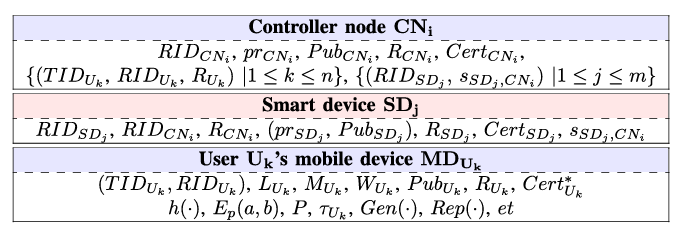
\includegraphics[width=0.8\linewidth]{pre-loaded.png} % Replace with actual figure file name
        \caption{Loaded Credentials in \( CNi \), \( SDj \), and User \( U_k \)'s Mobile Device \( \text{MD}_{U_k} \)}
    \end{figure}

\end{frame}

\subsection{D. Login Phase}
\begin{frame}
    \frametitle{D. Login Phase}
    \textbf{Step 1: User inputs data into mobile device and initial calculations.\\}
    \textbf{User \( U_k \) Login Attempt into ICPS environment}
    
    \begin{itemize}
        \item \( U_k \) inputs:
        \begin{itemize}
            \item Identity \( \text{ID}_{U_k} \)
            \item Password \( \text{PW}_{U_k} \)
            \item Personal biometrics \( \text{BM'}_{U_k} \)
        \end{itemize}
        
        \item \( \text{MD}_{U_k} \) performs calculations:
        \begin{itemize}
            \item Computes \( \sigma_{U_k} = \text{Rep}(\text{BM}_{U_k}, \tau_{U_k}) \) if the Hamming distance between registered and current biometric is within tolerance \( e_t'' \)
            \item Computes \( a^*_k = M_{U_k} \oplus h(\text{PW}_{U_k} || \sigma_{U_k} || \text{ID}_{U_k}) \)
            \item Generates pseudo-identity \( \text{PID}_{U_k} = h(\text{ID}_{U_k} || a^*_k) \)
            \item Determines private key \( \text{pr}_{U_k} = L_{U_k} \oplus h(\sigma_{U_k} || \text{PID}_{U_k} || \text{PW}_{U_k}) \)
            \item Computes \( \text{Cert'}_{U_k} = \text{Cert}^*_{U_k} \oplus h(\sigma_{U_k} || \text{PW}_{U_k}) \)
        \end{itemize}
    \end{itemize}

\end{frame}


\begin{frame}
    \frametitle{D. Login Phase}

    \textbf{Verification and Authentication Request Generation}

    \begin{itemize}
        \item \textbf{Step 2: Verification}
        \begin{itemize}
            \item \( \text{MD}_{U_k} \) calculates \( W^*_{U_k} = h(\text{Cert'}_{U_k} || \text{RID}_{U_k} || \text{PW}_{U_k} || \text{R}_{U_k} || \text{pr}_{U_k}) \)
            \item If \( W^*_{U_k} \neq W_{U_k} \), the session is aborted.
            \item Otherwise, it picks a random secret \( k_1 \in Z^*_p \) and generates timestamp \( \text{TS}_1 \).
            \item Computes:
            \begin{itemize}
                \item \( k_1' = h(k_1 || \text{pr}_{U_k} || \text{TS}_1) \)
                \item \( K_1' = k_1'.P \)
                \item \( \text{RID}^*_{SD_j} = \text{RID}_{SD_j} \oplus h(\text{R}_{U_k} || \text{RID}_{U_k} || \text{TS}_1) \)
                \item \( \text{Cert}^+_{U_k} = \text{Cert'}_{U_k} + h(\text{RID}^*_{SD_j} || \text{R}_{U_k} || K_1' || \text{Pub}_{U_k} || \text{TS}_1) \cdot k_1' (\mod p) \)
            \end{itemize}
            \item Generates a temporary identity \( \text{TID}_{U_k}^{\text{new}} \) and computes \( \text{TID}^*_{U_k} \)
            \item Computes:
            \begin{itemize}
                \item \( \text{TID}^*_{U_k} = \text{TID}_{U_k}^{\text{new}} \oplus h(\text{TID}_{U_k} || \text{RID}_{U_k} || \text{R}_{U_k} || \text{TS}_1) \)

                \item \( \text{TC}_{U_k} = h(\text{TS}_1 || \sigma_{U_k} || \text{PW}_{U_k} || \text{PID}_{U_k}) \)
                \item \( B_{U_k} = \text{TC}_{U_k} \oplus h(\text{RID}_{U_k} || \text{TS}_1 || \text{R}_{U_k}) \)
            \end{itemize}
        \end{itemize}

        \item \textbf{Step 3: Sending Authentication Request}
        \begin{itemize}
            \item \( \text{MD}_{U_k} \) sends \( \text{Msg}_1 = \langle \text{TID}_{U_k}, \text{TID}^*_{U_k}, \text{Cert}^+_{U_k}, K_1', \text{RID}^*_{SD_j}, B_{U_k}, \text{TS}_1 \rangle\)  to \( C_{N_i} \) via public channel.
        \end{itemize}
    \end{itemize}

\end{frame}
\subsection{E. Authentication and Key Agreement Phase}
\begin{frame}
    \frametitle{E. Authentication and Key Agreement Phase (Part 1)}

    \textbf{Controller Node \( C_{N_i} \) upon Receiving Authentication Request \( \text{Msg}_1 \):}

    \begin{itemize}
        \item \textbf{Step 1: Timestamp Verification}
        \begin{itemize}
            \item \( C_{N_i} \) checks if \( |\text{TS}_1 - \text{TS}^*_1| \leq \Delta T \), where \( \text{TS}^*_1 \) is the reception time of \( \text{Msg}_1 \).
            \item If the condition fails, \( C_{N_i} \) halts further processing.
            \item Otherwise, \( C_{N_i} \) retrieves \( (\text{RID}_{U_k}, \text{R}_{U_k}) \) for user \( U_k \) using \( \text{TID}_{U_k} \).
        \end{itemize}

        \item \textbf{Step 2: Authentication Verification}
        \begin{itemize}
            \item \( C_{N_i} \) verifies the below equation,  If it matches, \( C_{N_i} \) proceeds; otherwise, it aborts the process.
            \(
                \text{Pub}_{RA} + h(\text{RID}_{U_k} || \text{Pub}_{RA} || \text{Pub}_{U_k}) \cdot \text{R}_{U_k} + h(\text{RID}^*_{SD_j} || \text{R}_{U_k} || K_1' || \text{Pub}_{U_k} || \text{TS}_1) \cdot K_1' = \text{Cert}^+_{U_k} \cdot P
            \)
        \end{itemize}
    \end{itemize}

\end{frame}

\begin{frame}
    \frametitle{E. Authentication and Key Agreement Phase (Part 1)}


    \begin{itemize}

        \item \textbf{Step 3: Retrieve and Calculate Required Values}
        \begin{itemize}
            \item Retrieve \( \text{RID}_{SD_j} = \text{RID}^*_{SD_j} \oplus h(\text{R}_{U_k} || \text{RID}_{U_k} || \text{TS}_1) \)
            \begin{itemsize}
                \item \(\text{Cert'}_{C_{N_i}} &= \text{Cert}_{C_{N_i}} \oplus h(\text{TID}_{U_k} || s_{SD_j,C_{N_i}} || \text{TS}_2)\) 
                \item \(\text{TC}_{U_k} &= B_{U_k} \oplus h(\text{RID}_{U_k} || \text{TS}_1 || \text{R}_{U_k})\) 
                \item \(C_{U_k} &= h(\text{TC}_{U_k} || \text{TS}_2) \oplus h(s_{SD_j,C_{N_i}} || \text{TS}_2 || \text{TID}_{U_k} || \text{RID}_{SD_j})\) 
                \item \(X_i &= h(\text{TID}_{U_k} || s_{SD_j,C_{N_i}} || K_1' || C_{U_k} || \text{R}_{C_{N_i}} || \text{Cert'}_{C_{N_i}} || \text{RID}_{C_{N_i}} || \text{RID}_{SD_j} || \text{TS}_1 || \text{TS}_2)\)
            \end{itemsize}
            \item Send key establishment request \( \text{Msg}_2 = \langle \text{TID}_{U_k}, X_i, \text{Cert'}_{C_{N_i}}, K_1', C_{U_k}, \text{TS}_1, \text{TS}_2 \rangle \) to \( SD_j \).
        \end{itemize}

        \item \textbf{Step 4: Update Temporary Identity}
        \begin{itemize}
            \item Calculate \( \text{TID}_{U_k}^{\text{new}} = \text{TID}^*_{U_k} \oplus h(\text{TID}_{U_k} || \text{RID}_{U_k} || \text{R}_{U_k} || \text{TS}_1) \)
            \item Update \( \text{TID}_{U_k} \) with \( \text{TID}_{U_k}^{\text{new}} \) for \( U_k \) in \( C_{N_i} \)'s secure database.
        \end{itemize}
    \end{itemize}

\end{frame}

\begin{frame}
    \frametitle{E. Authentication and Key Agreement Phase (Part 2)}

    \textbf{Service Device \( SD_j \) upon Receiving Key Establishment Request \( \text{Msg}_2 \):}

    \begin{itemize}
        \item \textbf{Step 1: Timestamp Verification}
        \begin{itemize}
            \item \( SD_j \) checks if \( |\text{TS}_2 - \text{TS}^*_2| \leq \Delta T \), where \( \text{TS}^*_2 \) is the current timestamp at \( SD_j \). If the condition fails, \( SD_j \) discards the request as stale.
            \item Otherwise, \( SD_j \) retrieves \( (\text{RID}_{SD_j}, \text{RID}_{C_{N_i}}, s_{SD_j,C_{N_i}}) \) from memory and computes:\\
            \(
                \text{Cert}_{C_{N_i}} = \text{Cert'}_{C_{N_i}} \oplus h(\text{TID}_{U_k} || s_{SD_j,C_{N_i}} || \text{TS}_2)
            \)
        \end{itemize}

        \item \textbf{Step 2: Authentication Verification}
        \begin{itemize}
            \item Calculate:
            \(
                X^*_i = h(\text{TID}_{U_k} || s_{SD_j,C_{N_i}} || K_1' || C_{U_k} || \text{R}_{C_{N_i}} || \text{Cert}_{C_{N_i}} || \text{RID}_{C_{N_i}} || \text{RID}_{SD_j} || \text{TS}_1 || \text{TS}_2)
            \)
            \item Verify if \( X^*_i = X_i \) and:\\
            \(
                \text{Pub}_{RA} + h(\text{RID}_{C_{N_i}} || \text{Pub}_{RA} || \text{Pub}_{C_{N_i}}) \cdot \text{R}_{C_{N_i}} = \text{Cert}_{C_{N_i}} \cdot P
            \)
            \item If these conditions hold, \( SD_j \) authenticates \( C_{N_i} \) else terminates the session.
        \end{itemize}

        
    \end{itemize}

\end{frame}

\begin{frame}
    \frametitle{E. Authentication and Key Agreement Phase (Part 2)}


    \begin{itemize}
       
        \item \textbf{Step 3: Session Key Computation}
        \begin{itemize}
            \item \( SD_j \) picks a random secret \( k_2 \in Z^*_p \) and computes:
            \begin{align*}
                k_2' &= h(k_2 || s_{SD_j,C_{N_i}} || \text{pr}_{SD_j} || \text{TS}_3) \\
                K_2' &= k_2' \cdot P \\
                \text{Cert}^+_{SD_j} &= \text{Cert}_{SD_j} + h(\text{TID}_{U_k} || \text{RID}_{SD_j} || K_2' || \text{Pub}_{SD_j} || \text{TS}_3) \cdot k_2' (\mod p)
            \end{align*}
            \( h(\text{TC}_{U_k} || \text{TS}_2) = C_{U_k} \oplus h(s_{SD_j, C_{N_i}} || \text{TS}_2 || \text{TID}_{U_k} || \text{RID}_{SD_j}) \)

            \item Calculate the shared session key:
            \[
                \text{SK}_{SD_j,U_k} = h(k_2' \cdot K_1' || h(\text{TC}_{U_k} || \text{TS}_2) || \text{RID}_{SD_j} || \text{TID}_{U_k} || \text{TS}_1 || \text{TS}_3)
            \]
            \item Compute session key verifier:
            \[
                \text{SKV} = h(\text{SK}_{SD_j,U_k} || \text{TS}_2 || \text{TS}_3)
            \]
        \end{itemize}

        \item \textbf{Step 4: Sending Key Establishment Response}
        \begin{itemize}
            \item \( SD_j \) sends the key establishment response \( \text{Msg}_3 = \langle \text{Cert}^+_{SD_j}, \text{R}_{SD_j}, K_2', \text{SKV}, \text{TS}_2, \text{TS}_3 \rangle \) to \( U_k \) via a public channel.
        \end{itemize}
    \end{itemize}

\end{frame}

\begin{frame}
    \frametitle{E. Authentication and Key Agreement Phase (Part 3)}

    \textbf{User \( U_k \) Session Key Establishment with \( SD_j \)}

    
    \text After receiving \(\text{Msg}_3\) from \( SD_j \), \( \text{MD}_{U_k} \) performs the following operations:
        \begin{itemize}
            \item \textbf{Step 1: Timestamp Verification:}
            \begin{itemize}
                \item \( \text{MD}_{U_k} \) verifies the freshness of the message by checking if \( |\text{TS}_3 - \text{TS}^*_3| \leq \Delta T \), where \( \text{TS}^*_3 \) is the current timestamp generated by \( U_k \).
                \item If the condition is not met, \( U_k \) discards the response and stops further processing.
            \end{itemize}

            \item \textbf{Step 2: Signature Verification:}
            \begin{itemize}
                \item \( \text{MD}_{U_k} \) checks the validity of the signature:
                \(
                \text{Pub}_{RA} + h(\text{RID}_{SD_j} || \text{Pub}_{RA} || \text{Pub}_{C_{N_i}} || \text{Pub}_{SD_j}) \cdot \text{R}_{SD_j} + h(\text{TID}_{U_k} || \text{RID}_{SD_j} || K_2' || \text{Pub}_{SD_j} || \text{TS}_3) \cdot K_2' = \text{Cert}^+_{SD_j} \cdot P
                \)
                \item If this condition fails, \( U_i \) discards the response and stops the session.
            \end{itemize}

            
        \end{itemize}
   
\end{frame}

\begin{frame}
    \frametitle{E. Authentication and Key Agreement Phase (Part 3)}

    \textbf{User \( U_k \) Session Key Establishment with \( SD_j \)}

    
        \begin{itemize}
            
            \item \textbf{Step 3: Session Key Computation:}
            \begin{itemize}
                \item \( \text{MD}_{U_k} \) computes the session key:
                \[
                \text{SK}_{U_k, SD_j} = h(k_1' \cdot K_2' || h(\text{TC}_{U_k} || \text{TS}_2) || \text{RID}_{SD_j} || \text{TID}_{U_k} || \text{TS}_1 || \text{TS}_3)
                \]
                \item Computes the session key verifier:
                \[
                \text{SKV}^* = h(\text{SK}_{U_k, SD_j} || \text{TS}_2 || \text{TS}_3)
                \]
                \item \( \text{MD}_{U_k} \) checks if \( \text{SKV}^* = \text{SKV} \). If invalid, \( U_k \) aborts the session. Otherwise, \( U_k \) and \( SD_j \) successfully establish the session key.
            \end{itemize}

            \item \textbf{Step 4: Identity Update:}
            \begin{itemize}
                \item \( U_k \) updates \( \text{TID}_{U_k} \) with \( \text{TID}_{U_k}^{\text{new}} \) in \( \text{MD}_{U_k} \).
                \item The overall phase is summarized in the image next slide.
            \end{itemize}
        \end{itemize}
    
\end{frame}

\begin{frame}
    \frametitle{E. Login and Authentication and Key Agreement Phases}
    
    \begin{figure}
        \centering
        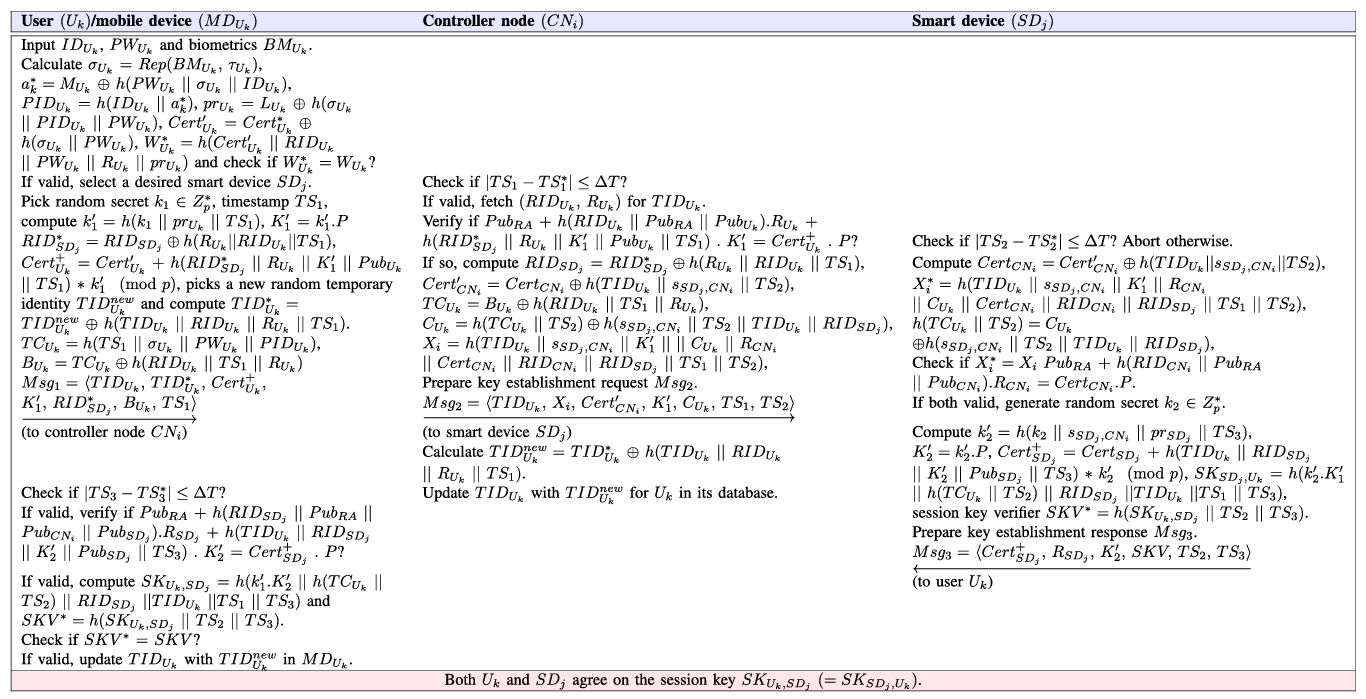
\includegraphics[width=\textwidth]{Esteap.png} 
        \caption{Login and authentication and key agreement phases.}
    \end{figure}
\end{frame}

\subsection{F. User Credentials Update Phase}
\begin{frame}
    \frametitle{F. User Credentials Update Phase (Part 1)}

    \textbf{Overview:} Registered user \( U_k \) may wish to change credentials, such as password or biometrics. This phase facilitates updating any or all credentials: \emph{identity} \( \text{ID}_{U_k} \), \emph{password} \( \text{PW}_{U_k} \), and \emph{biometrics} \( \text{BM}_{U_k} \).

    \begin{itemize}
        \item \textbf{Step 1: Input Current Credentials}
        \begin{itemize}
            \item \( U_k \) inputs current credentials \( \text{ID}_{U_k}^{\text{cur}}, \text{PW}_{U_k}^{\text{cur}} \), and biometrics \( \text{BM}_{U_k}^{\text{cur}} \) into \( \text{MD}_{U_k} \).
            \item \( \text{MD}_{U_k} \) computes \( \sigma_{U_k}^{\text{cur}} = \text{Rep}(\text{BM}_{U_k}^{\text{cur}}, \tau_{U_k}) \).
            \item Calculates \( a^*_k = M_{U_k} \oplus h(\text{PW}_{U_k}^{\text{cur}} || \sigma_{U_k}^{\text{cur}} || \text{ID}_{U_k}^{\text{cur}}) \).
            \item Derives:
            \begin{itemize}
                \item \( \text{PID}_{U_k}^{\text{cur}} = h(\text{ID}_{U_k}^{\text{cur}} ||  a^*_k) \)
                \item \( \text{pr}_{U_k}^* = L_{U_k} \oplus h(\sigma_{U_k}^{\text{cur}} || \text{PID}_{U_k}^{\text{cur}} || \text{PW}_{U_k}^{\text{cur}} ) \)
                \item \( \text{Cert}_{U_k}^* = \text{Cert}_{U_k} \oplus h(\sigma_{U_k}^{\text{cur}}  || \text{PW}_{U_k}^{\text{cur}}) \)
            \end{itemize}
            \item Checks if \( W_{U_k} = h(\text{Cert}_{U_k}^* || \text{RID}_{U_k} || \text{PW}_{U_k}^{\text{cur}} || \text{R}_{U_k} || \text{pr}_{U_k}^*) \) if it doesn't satisfy it stops proceeding further.
        \end{itemize}
        
       
    \end{itemize}
    
    \vspace{0.5em}
\end{frame}

\begin{frame}
    \frametitle{F. User Credentials Update Phase (Part 2)}

    \begin{itemize}
        
        \item \textbf{Step 2: Input New Credentials}
        \begin{itemize}
            \item \( U_k \) inputs new credentials \( \text{ID}_{U_k}^{\text{new}}, \text{PW}_{U_k}^{\text{new}}, \text{BM}_{U_k}^{\text{new}} \).
            \item \( \text{MD}_{U_k} \) computes:
            \begin{itemize}
                \item \( \sigma_{U_k}^{\text{new}}, \tau_{U_k}^{\text{new}} = \text{Gen}(\text{BM}_{U_k}^{\text{new}}) \)
                \item \( \text{PID}_{U_k}^{\text{new}} = h(\text{ID}_{U_k}^{\text{new}} ||  a^*_k) \)
                \item \( L_{U_k}^{\text{new}} = \text{pr}_{U_k}^* \oplus h(\sigma_{U_k}^{\text{new}} || \text{PID}_{U_k}^{\text{new}} || \text{PW}_{U_k}^{\text{new}} ) \)
                \item \( M_{U_k}^{\text{new}} = a^*_k \oplus h(\text{PW}_{U_k}^{\text{new}} || \sigma_{U_k}^{\text{new}} || \text{ID}_{U_k}^{\text{new}}) \)
                
                \item \( \text{Cert}_{U_k}^{\text{new}} = \text{Cert}_{U_k}^* \oplus h(\sigma_{U_k}^{\text{new}} || \text{PW}_{U_k}^{\text{new}}) \)
                \item \( W_{U_k}^{\text{new}} = h(\text{Cert}_{U_k}^{\text{new}}^* || \text{RID}_{U_k} || \text{PW}_{U_k}^{\text{new}} || \text{R}_{U_k} || \text{pr}_{U_k}^*) \)
            \end{itemize}
        \end{itemize}
        
        \item \textbf{Step 3: Update and Replace}
        \begin{itemize}
            \item \( \text{MD}_{U_k} \) replaces \( L_{U_k}, M_{U_k}, \text{Cert}_{U_k}, W_{U_k}, \tau_{U_k} \) with the new values: \( L_{U_k}^{\text{new}}, M_{U_k}^{\text{new}}, \text{Cert}_{U_k}^{\text{new}}, W_{U_k}^{\text{new}}, \tau_{U_k}^{\text{new}} \).
        \end{itemize}
    \end{itemize}
    
    \vspace{0.5em}
    \textit{The summary of this phase is provided in Figure next slide}
\end{frame}
\begin{frame}
    \frametitle{User Credentials Update Phase}

    \begin{figure}
        \centering
        
        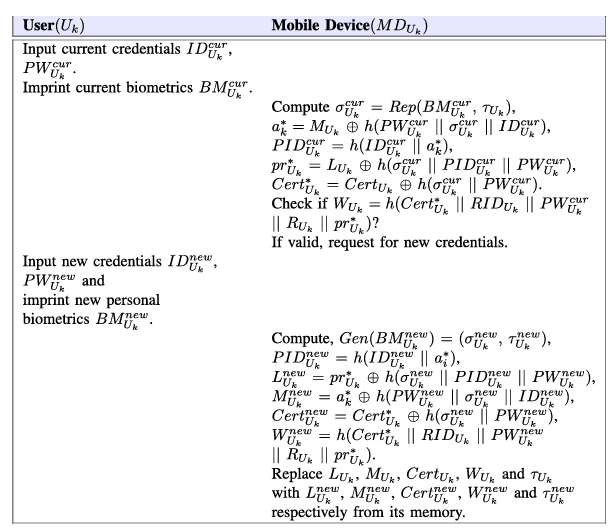
\includegraphics[width=0.8\textwidth]{fig4.png}
        \caption{User credentials update phase.}
        \label{fig:user_credentials_update}
    \end{figure}

\end{frame}

\subsection{G. Dynamic Smart Device Addition Phase}
\begin{frame}
    \frametitle{G. Dynamic Smart Device Addition Phase}

    The proposed scheme allows adding new smart devices to an ICPS post-deployment and further participating in the authentication and key agreement phase to establish secure sessions with a user \( U_k \). The RA performs the following steps to add a new smart device \( SD_n \):

    \begin{itemize}
        \item \textbf{Step 1:} 
        \begin{itemize}
            \item Generate a pseudo-identity \( RID_{SD_n} = h(ID_{SD_n} || pr_{RA}) \).
            \item Randomly choose a secret \( r_{SD_n} \in Z^*_p \) to compute \( R_{SD_n} = r_{SD_n}.P \).
            \item Prepare a personalized private-public key pair \( (pr_{SD_n}, Pub_{SD_n}) \) by randomly selecting \( pr_{SD_n} \in Z^*_p \) and computing \( Pub_{SD_n} = pr_{SD_n}.P \).
        \end{itemize}
        
       
    \end{itemize}


\end{frame}

\begin{frame}
    \frametitle{G. Dynamic Smart Device Addition Phase}
    \begin{itemize}
        
        
        \item \textbf{Step 2:} 
        \begin{itemize}
            \item Generate a certificate 
            \[
            Cert_{SD_n} = \left( pr_{RA} + h(RID_{SD_n} || Pub_{RA} || Pub_{CNi} || Pub_{SD_n}) \cdot r_{SD_n} \right) (\mod p).
            \]
            \item Generate the shared secret 
            \[
            s_{SD_n,CNi} = h(RID_{SD_n} || RID_{CNi} || r_{SD_n} || r_{CNi} || RT_{SD_n}).
            \]
            \item Send the tuple \( (RID_{SD_n}, s_{SD_n,CNi}) \) to \( C_{Ni} \) via a secure channel.
        \end{itemize}

        \item \textbf{Step 3:} 
        \begin{itemize}
            \item Load \( \{RID_{SD_n}, RID_{CNi}, R_{CNi}, pr_{SD_n}, Pub_{SD_n}, R_{SD_n}, Cert_{SD_n}, s_{SD_n,CNi}\} \) into the memory of \( SD_n \) and deploy it in the ICPS environment.
            \item RA erases \( ID_{SD_n}, RT_{SD_n}, r_{SD_n}, \) and \( pr_{SD_n} \) from memory.
        \end{itemize}
    \end{itemize}

    The overall phase is summarized in the figure next slide.

\end{frame}

\begin{frame}
    \frametitle{G. Dynamic Smart Device Addition Phase}

    \begin{figure}
        \centering
        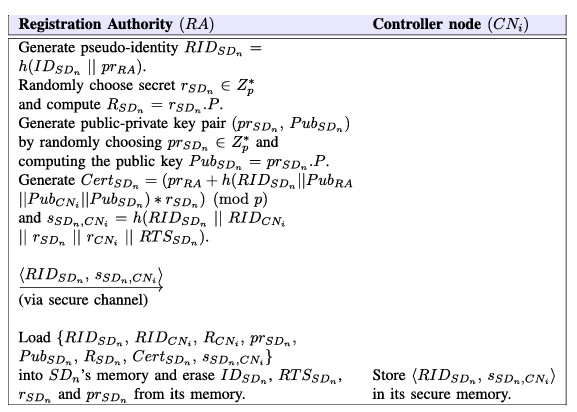
\includegraphics[width=0.8\textwidth]{Fig5.png} 
        \caption{Dynamic smart device (SDn) addition phase.}
        \label{fig:SDn_addition_phase}
    \end{figure}

\end{frame}

\section{Security Analysis}
\begin{frame}
    \frametitle{IV. Security Analysis}
    \begin{itemize}
        \item Discussion on the resilience of the proposed scheme (UAKA-5GSICPS) against various attacks.
        \item Focus on the formal security analysis under the Random Oracle (ROR) model.
    \end{itemize}
\end{frame}
\subsection{A. Formal Security Analysis Under ROR Model}
\begin{frame}
    \frametitle{A. Formal Security Analysis Under ROR Model}
    \begin{itemize}
        \item Analysis through Random Oracle (ROR) model to prove:
            \begin{itemize}
                \item Semantic security
                \item Session key security (SK-security)
            \end{itemize}
        \item Discussion on the ROR model and the SK-security of the proposed scheme in Theorem 1.
    \end{itemize}
\end{frame}

\begin{frame}
    \frametitle{Entities and Hash Function in the ROR Model}
    \begin{itemize}
        \item Entities representation:
            \begin{itemize}
                \item User: \( \text{\large $\varepsilon$}_{Uk} \)
                \item Controller Node: \( \text{\large $\varepsilon$}_{CNi} \)
                \item Smart Device: \( \text{\large $\varepsilon$}_{SDj} \)
            \end{itemize}
        \item Instances representation:
            \begin{itemize}
                \item \( \text{\large $\varepsilon$}_{t1}^{Uk} \), \( \text{\large $\varepsilon$}_{t2}^{CNi} \), \( \text{\large $\varepsilon$}_{t3}^{SDj} \)
            \end{itemize}
         \item Collision-resistant one-way hash function \( h(.) \):
            \begin{itemize}
                \item Modeled as a random oracle \( H \)
                \item Publicly available to all entities in the ROR model
            \end{itemize}
    \end{itemize}
\end{frame}





\begin{frame}
    \frametitle{Adversary Queries}
    \begin{itemize}
        \item List of queries for the adversary \( A \):
            \begin{itemize}
                \item \textbf{\(Q_{Read}(\varepsilon_{t1}^{Uk}, \varepsilon_{t2}^{CNi}, \varepsilon_{t3}^{SDj})\)}: 
                An adversary \( A \) uses this query to eavesdrop the publicly exchanged messages \( Msg1, Msg2, Msg3 \) among \( \varepsilon_{t1}^{Uk}, \varepsilon_{t2}^{CNi}, \) and \( \varepsilon_{t3}^{SDj} \) during the authentication and session key establishment. This is analogous to an “eavesdropping attack”.
                \item \textbf{\(Q_{Send}(\varepsilon_{t}, Msg)\)}: 
                This query allows \( A \) to send a message \( Msg \) to \( \varepsilon_{t} \) and in turn receive the response from \( \varepsilon_{t} \). It is analogous to an “active attack”.
                \item \textbf{\(Q_{CorruptMD}(\varepsilon_{t1}^{Uk})\)}: 
                By querying this, \( A \) can extract the parameters of \( MD_{Uk} \), which is the registered mobile device of a user \( Uk \). This is analogous to an “active attack”.
                \item \textbf{\(Q_{RevealSK}(\varepsilon_{t})\)}: 
                With this query, the shared secret session key \( SK_{Uk,SDj} = (SK_{SDj,Uk}) \) between \( Uk \) and \( SDj \) is revealed to the adversary \( A \).
                \item \textbf{\(Q_{Test}(\varepsilon_{t})\)}: 
                The output of this query is based on the outcome of an unbiased coin “\( c \)”:
                \begin{itemize}
                    \item If “Flip(c) = HEAD”, it returns the shared session key \( SK_{Uk,SDj} \) between \( Uk \) and \( SDj \), if it is freshly generated.
                    \item If “Flip(c) = TAIL”, it randomly selects the session key \( SK_{Uk,SDj} \in Z^*_p \) and returns \( SK_{Uk,SDj} \).
                \end{itemize}
            \end{itemize}
    \end{itemize}
\end{frame}


\begin{frame}
    \frametitle{Application of Zipf’s Law \cite{Wang2017}}
    \begin{itemize}
        \item User passwords are not uniformly distributed.
        \item Application of Zipf’s law to prove SK-security of UAKA-5GSICPS.
    \end{itemize}
\end{frame}

\begin{frame}
    \frametitle{Theorem 1}
    \begin{itemize}
        \item Let \( Adv_{A}^{UAKA \− 5GSICPS}(t) \) be the advantage function of adversary \( A \) running in polynomial time t:
            \begin{itemize}
                \item Definitions:
                    \begin{itemize}
                        \item \( q_h \): Number of Hash queries
                        \item \( q_r \): Number of Read queries
                        \item \( |H| \): Range space of \( h(.) \)
                        \item \( Adv_{A}^{ECDDHP}(t) \): Advantage of breaking the ECDDHP
                        \item \( l_\sigma \): Number of bits in the biometric secret key \( \sigma_{Uk} \)
                        \item \( C', s' \): Zipf’s parameters
                    \end{itemize}
                \item Result: 
                \[
                Adv_{A}^{UAKA−5GSICPS}(t) \leq \frac{q_h^2}{|H|} + 2\left[\max\{C' \cdot q_r^{s'} , \frac{q_r}{2^{l_\sigma}}\} + Adv_A^{ECDDHP}(t)\right]
                \]
            \end{itemize}
    \end{itemize}
\end{frame}

\begin{frame}
    \frametitle{Proof Outline}
    \begin{itemize}
        \item Follows a similar proof structure as in \cite{Chatterjee2018, Roy2018, Wazid2020}.
        \item Define four games: \( G_0, G_1, G_2, G_3 \).
        \item Event \( Succ_A^{G_j} \): Adversary correctly guesses the coin flip outcome.
        \item Advantage of winning the game:
        \[
        Adv_A^{G_j} = Pr[Succ_A^{G_j}]
        \]
    \end{itemize}
\end{frame}
\begin{frame}
    \frametitle{Game G_0}
    \begin{itemize}
        \item \textbf{Description}: This game corresponds to the actual attack executed by adversary \( A \) against our proposed protocol in the ROR model.
        \item \textbf{Key Definition}: The outcome of the coin flip \( c \) is selected randomly at the beginning of \( G_0 \).
        \item \textbf{Advantage Calculation}:
        \[
            Adv_{A}^{UAKA-5GSICPS} = |2 \cdot Adv_{A}^{G_0} - 1|
        \]
    \end{itemize}
\end{frame}
\begin{frame}
    \frametitle{Game G_1}
    \begin{itemize}
        \item \textbf{Description}: Modeled as an “eavesdropping attack” where \( A \) tries to read public messages exchanged during the authentication and key agreement phase.
        \item \textbf{Messages Involved}:
            \begin{itemize}
                \item \( Msg_1 = \langle TID_{Uk}, TID^{*}_{Uk}, Cert^{+}_{Uk}, K_1', RID^{*}_{SDj}, BU_{k}, TS_1 \rangle \)
                \item \( Msg_2 = \langle TID_{Uk}, X_i, Cert_{CNi}', K_1', CU_{k}, TS_1, TS_2 \rangle \)
                \item \( Msg_3 = \langle Cert^{+}_{SDj}, R_{SDj}, K_2', SK_{V}, TS_2, TS_3 \rangle \)
                \item Sent from \( U_k \) to \( C_{Ni} \), \( C_{Ni} \) to \( SD_j \), and \( SD_j \) to \( U_k \), respectively, during the authentication and key agreement phase III-E using \( Q_{Read} \) query.
            \end{itemize}
        \item \textbf{Query Usage}: Adversary invokes \( Q_{Read} \) to read messages and later invokes \( Q_{RevealSK} \) and \( Q_{Test} \) to check if the session key \( SK_{Uk,SDj} \) is a legitimate key or a random number
        \(
            SK_{SDj,Uk} = h(k_2' \cdot K_1' \parallel h(TC_{Uk} \parallel TS_2) \parallel RID_{SDj} \parallel TID_{Uk} \parallel TS_1 \parallel TS_3) = h(k_1' \cdot K_2' \parallel h(TC_{Uk} \parallel TS_2) \parallel RID_{SDj} \parallel TID_{Uk} \parallel TS_1 \parallel TS_3) = SK_{Uk,SDj}
        \)
        Hence, the adversary \( A \) cannot distinguish a valid session key \( SK_{SDj,Uk} \) from a random number.
        \item \textbf{Indistinguishability}: Since \( G_0 \) and \( G_1 \) are indistinguishable,
        \[
            Adv_{A}^{G_1} = Adv_{A}^{G_0}
        \]
    \end{itemize}
\end{frame}

\begin{frame}
    \frametitle{Game G_2}
    \begin{itemize}
        \item \textbf{Description}: Models an “active attack” by simulating the H oracle.
        \item \textbf{Security Properties}:
            \begin{itemize}
                \item Messages \( Msg_1, Msg_2, Msg_3 \) are protected with the collision-resistant one-way hash function \( h(.) \).
                \item Extracting sensitive parameters is computationally infeasible due to the one-way property of \( h(.) \).
                \item The values \( TID^{*}_{Uk}, Cert^{+}_{Uk}, RID^{*}_{SDj}, X_i, Cert_{CNi}, Cert^{+}_{SDj}, SK_{V} \) included in the network messages are indistinguishable.
                \item Due to the inclusion of timestamps \( TS_k \) where \( k \in [1, 3] \), and the short-term keys \( k_1 \) and \( k_2 \) (which are for one-time use), collision resistance is assured.
            \end{itemize}
        \item \textbf{Indistinguishability}: \( G_1 \) and \( G_2 \) are indistinguishable, except that \( G_2 \) includes the H query simulation.
        \item \textbf{Advantage Relation}:
        \[
            |Adv_{A}^{G_1} - Adv_{A}^{G_2}| \leq \frac{q^2}{2|H|} + Adv_{A}^{ECDHP}(t)
        \]
    \end{itemize}
\end{frame}


\begin{frame}
    \frametitle{Game G_3}
    \begin{itemize}
        \item \textbf{Description}: The adversary \( A \) attempts to tamper with the smart device \( MD_{Uk} \) of a user \( U_k \) using \( Q_{CorruptMD} \).
        \item \textbf{Challenges for A}:
            \begin{itemize}
                \item Extracting sensitive parameters is computationally infeasible without knowing \( ID_{Uk}, PW_{Uk}, \sigma_{Uk} \).
                \item The probability of guessing the biometric key \( \sigma_{Uk} \) is approximately \( \frac{1}{2^{l_{\sigma}}} \).
            \end{itemize}
        \item \textbf{Indistinguishability}: \( G2 \) and \( G3 \) are identical with no password/biometric guessing attacks.
        \item \textbf{Advantage Relation}: Hence,with the Zipf’s law on passwords \cite{Wang2017}, we have: 
        \[
            |Adv_{A}^{G_2} - Adv_{A}^{G_3}| \leq \max\{C' \cdot q_r^{s'}, \frac{q_r}{2^{l_\sigma}} \}
        \]
        \item using all the equations from the previous games we get:
        \[
            Adv_{A}^{UAKA-5GSICPS}(t) \leq \frac{q_h^2}{|H|} + 2\left[\max\{C' \cdot q_r^{s'} , \frac{q_r}{2^{l_\sigma}}\} + Adv_A^{ECDDHP}(t)\right]
        \]
    \end{itemize}
\end{frame}

\subsection{B. Informal Security Analysis}
\begin{frame}
    \frametitle{Informal Security Analysis}
    In this section, we demonstrate that the proposed scheme possesses the ability to resist various potential attacks. 
    The following informal methods highlight the robustness of the system against specific threats:
\end{frame}

\begin{frame}
    \frametitle{1. User Impersonation Attack}
    \begin{itemize}
        \item \textbf{Attack Overview}:
            \begin{itemize}
                \item An adversary \( A \) attempts to impersonate a legitimate user \( U_k \) by crafting a valid authentication request.
                \item Required message format: 
                \[
                Msg_1 = TID_{U_k}, TID^{*}_{U_k}, Cert^{+}_{U_k}, K_1, RID^{*}_{SD_j}, B_{U_k}, TS_1
                \]
            \end{itemize}
        \item \textbf{Adversary Capabilities}:
            \begin{itemize}
                \item \( A \) can generate a random secret \( k_A \) and compute \( K_A = k_A \cdot P \).
                \item The timestamp \( TS_A \) can be selected as the time of sending the fabricated message.
            \end{itemize}
        \item \textbf{Limitations of \( A \)}:
            \begin{itemize}
                \item Cannot generate a valid certificate \( Cert^{+}_{U_k} \) due to unknown parameters \( R_{U_k}, RID_{U_k}, Cert_{U_k}, pr_{U_k} \).
                \item Even if \( A \) captures the user’s smart device \( MD_{U_k} \), the parameters \( Cert_{U_k} \) and \( pr_{U_k} \) are masked using \( PID_{U_k}, PW_{U_k}, \sigma_{U_k} \).
                \item The adversary cannot fabricate \( TID^{*}_{U_k} \) due to unknown values \( RID_{U_k} \) and \( R_{U_k} \).
            \end{itemize}
        \item \textbf{Conclusion}:
            \begin{itemize}
                \item Therefore, \( A \) cannot impersonate a registered user in UAKA-5GSICPS.
            \end{itemize}
    \end{itemize}
\end{frame}

\begin{frame}
    \frametitle{2. Controller Node Impersonation Attack}
    \begin{itemize}
        \item \textbf{Attack Overview}:
            \begin{itemize}
                \item An adversary \( A \) tries to impersonate a controller node \( C_{N_i} \) by sending a fabricated message.
                \item Required message format:
                \[
                Msg_2 = TID_{U_k}, X_i, Cert_{C_{N_i}}, K_1, C_{U_k}, TS_1, TS_2
                \]
            \end{itemize}
        \item \textbf{Adversary Capabilities}:
            \begin{itemize}
                \item \( A \) attempts to compute a valid \( X_i \) based on:
                \[
                X_i = h(TID_{U_k} || s_{SD_j,C_{N_i}} || K_1 || C_{U_k} || R_{C_{N_i}} || Cert_{C_{N_i}} || RID_{C_{N_i}} || RID_{SD_j} || TS_1 || TS_2)
                \]
            \end{itemize}
        \item \textbf{Limitations of \( A \)}:
            \begin{itemize}
                \item Cannot compute \( X_i \) due to unknown shared secret \( s_{SD_j,C_{N_i}} \).
                \item Even if \( A \) compromises \( SD_j \) and extracts \( s_{SD_j,C_{N_i}} \), the shared secret is distinct for each device, limiting the impact.
                \item Compromising \( SD_j \) does not expose sensitive information of other devices or registered users.
            \end{itemize}
        \item \textbf{Conclusion}:
            \begin{itemize}
                \item The scheme effectively withstands impersonation attempts against the controller node.
            \end{itemize}
    \end{itemize}
\end{frame}
\begin{frame}
    \frametitle{3. Smart Device Impersonation Attack}
    \begin{itemize}
        \item \textbf{Attack Overview}:
            \begin{itemize}
                \item The adversary \( A \) attempts to impersonate a smart device \( SD_j \) by fabricating an authentication response message.
                \item Required message format:
                \[
                Msg_3 = Cert^{+}_{SD_j}, R_{SD_j}, K_2, SK_V, TS_2, TS_3
                \]
            \end{itemize}
        \item \textbf{Adversary Capabilities}:
            \begin{itemize}
                \item \( A \) seeks to generate a valid \( Cert^{+}_{SD_j} \).
                \item Requires knowledge of:
                \[
                Cert_{SD_j} = (pr_{RA} + h(RID_{SD_j} || Pub_{RA} || Pub_{C_{N_i}} || Pub_{SD_j}) \cdot r_{SD_j}) \mod p
                \]
            \end{itemize}
        \item \textbf{Limitations of \( A \)}:
            \begin{itemize}
                \item Cannot extract \( Cert_{SD_j} \) without compromising \( SD_j \).
                \item Compromising \( SD_j \) does not impact the entire ICPS environment or expose critical information about other nodes and users.
            \end{itemize}
        \item \textbf{Conclusion}:
            \begin{itemize}
                \item The proposed scheme is resilient against smart device impersonation attacks.
            \end{itemize}
    \end{itemize}
\end{frame}

\begin{frame}
    \frametitle{4. User Anonymity and Untraceability}
    \begin{itemize}
        \item \textbf{Attack Overview}:
            \begin{itemize}
                \item The proposed scheme maintains user anonymity and untraceability during the login and authentication phases.
                \item User's real identity \( ID_{U_k} \) is never included in network messages.
            \end{itemize}
        \item \textbf{Adversary Capabilities}:
            \begin{itemize}
                \item Assume \( A \) collects the authentication request:
                \[
                Msg_1 = TID_{U_k}, TID^{*}_{U_k}, Cert^{+}_{U_k}, K_1, RID^{*}_{SD_j}, B_{U_k}, TS_1
                \]
                \item \( A \) captures the mobile device \( MD_{U_k} \) and extracts values such as \( TID_{U_k}, RID_{U_k}, L_{U_k}, M_{U_k}, W_{U_k}, Pub_{U_k}, R_{U_k}, Cert^{*}_{U_k}, h(\cdot), \) etc.
            \end{itemize}
        \item \textbf{Limitations of \( A \)}:
            \begin{itemize}
                \item Due to the collision-resistant property of the hash function \( h(\cdot) \), guessing \( ID_{U_k} \) from \( L_{U_k} \) and \( M_{U_k} \) is infeasible without knowledge of \( pr_{U_k}, PW_{U_k}, \sigma_{U_k}, \) and \( a_k \).
                \item Authentication requests from the same user are untraceable as \( TID_{U_k} \) differs for each request.
            \end{itemize}
        \item \textbf{Conclusion}:
            \begin{itemize}
                \item UAKA-5GSICPS ensures both user anonymity and untraceability, even if the registered mobile device \( MD_{U_k} \) is compromised or stolen.
            \end{itemize}
    \end{itemize}
\end{frame}

\begin{frame}
    \frametitle{5. Privileged Insider Attack}
    \begin{itemize}
        \item \textbf{Attack Overview}:
            \begin{itemize}
                \item Insider adversary \( A \) reads user registration request \( PID_{U_k}, Pub_{U_k} \) sent to the Registration Authority (RA).
                \item \( A \) accesses the registered user’s mobile device \( MD_{U_k} \) post-registration.
            \end{itemize}
        \item \textbf{Adversary Capabilities}:
            \begin{itemize}
                \item \( A \) can extract stored credentials from \( MD_{U_k} \).
                \item \( A \) cannot guess \( ID_{U_k} \) or \( a_k \) due to the collision-resistant hash function \( h(\cdot) \).
            \end{itemize}
        \item \textbf{Limitations of \( A \)}:
            \begin{itemize}
                \item \( A \) cannot deduce sensitive parameters \( pr_{U_k}, a_k, Cert_{U_k} \) without \( ID_{U_k}, PW_{U_k}, \sigma_{U_k} \).
            \end{itemize}
        \item \textbf{Conclusion}:
            \begin{itemize}
                \item The proposed scheme is resilient to privileged insider attacks, ensuring user security.
            \end{itemize}
    \end{itemize}
\end{frame}
\begin{frame}
    \frametitle{6. Stolen Registered Mobile Device Attack}
    \begin{itemize}
        \item \textbf{Attack Overview}:
            \begin{itemize}
                \item An adversary \( A \) steals the mobile device \( MD_{U_k} \) of a registered user \( U_k \).
            \end{itemize}
        \item \textbf{Adversary Capabilities}:
            \begin{itemize}
                \item \( A \) can access the device but cannot derive sensitive attributes \( a_k, pr_{U_k}, Cert_{U_k} \) without knowing \( ID_{U_k}, PW_{U_k}, \sigma_{U_k} \).
            \end{itemize}
        \item \textbf{Limitations of \( A \)}:
            \begin{itemize}
                \item Any modification of \( R_{U_k} \) or \( TID_{U_k} \) results in validation failures during authentication.
            \end{itemize}
        \item \textbf{Conclusion}:
            \begin{itemize}
                \item The proposed scheme protects sensitive information even in the case of a stolen mobile device.
            \end{itemize}
    \end{itemize}
\end{frame}

\begin{frame}
    \frametitle{7. Physical Smart Device Capture Attack}
    \begin{itemize}
        \item \textbf{Attack Overview}:
            \begin{itemize}
                \item An adversary \( A \) captures a smart device \( SD_j \) and extracts stored values.
            \end{itemize}
        \item \textbf{Adversary Capabilities}:
            \begin{itemize}
                \item \( A \) retrieves various parameters unique to \( SD_j \).
                \item Parameters \( k_2, K_1, TID_{U_k}, TS_1, \) and \( TS_3 \) are session-specific and independent.
            \end{itemize}
        \item \textbf{Limitations of \( A \)}:
            \begin{itemize}
                \item Compromising \( SD_j \) does not reveal session keys for other devices; only the session key for the compromised device is affected.
            \end{itemize}
        \item \textbf{Conclusion}:
            \begin{itemize}
                \item The proposed scheme maintains security against physical device capture attacks.
            \end{itemize}
    \end{itemize}
\end{frame}

\begin{frame}
    \frametitle{8. Password Guessing Attacks}
    \begin{itemize}
        \item \textbf{Attack Overview}:
            \begin{itemize}
                \item An adversary \( A \) attempts to guess the user’s password \( PW_{U_k} \) through various means.
            \end{itemize}
        \item \textbf{Adversary Capabilities}:
            \begin{itemize}
                \item \( A \) can capture \( MD_{U_k} \) and attempt to extract values, but cannot guess \( PW_{U_k} \) without additional information.
            \end{itemize}
        \item \textbf{Limitations of \( A \)}:
            \begin{itemize}
                \item The password is never transmitted over the network, making online guessing attacks infeasible.
                \item Deriving \( pr_{U_k} \) from \( Pub_{U_k} \) relies on the hardness of the ECDLP.
            \end{itemize}
        \item \textbf{Conclusion}:
            \begin{itemize}
                \item The proposed scheme is secure against both online and offline password guessing attacks.
            \end{itemize}
    \end{itemize}
\end{frame}
\begin{frame}
    \frametitle{9. Replay Attack}
    \begin{itemize}
        \item \textbf{Attack Overview}:
            \begin{itemize}
                \item An adversary \( A \) attempts to replay previously captured messages during authentication.
            \end{itemize}
        \item \textbf{Adversary Capabilities}:
            \begin{itemize}
                \item \( A \) captures messages that include timestamps to authenticate sessions.
            \end{itemize}
        \item \textbf{Limitations of \( A \)}:
            \begin{itemize}
                \item Messages are validated against their timestamps, ensuring freshness and preventing replay.
                \item Messages older than the maximum transmission delay \( T \) are rejected.
            \end{itemize}
        \item \textbf{Conclusion}:
            \begin{itemize}
                \item The proposed scheme effectively protects against replay attacks through timestamp validation.
            \end{itemize}
    \end{itemize}
\end{frame}

\begin{frame}
    \frametitle{10. Man-in-the-Middle (MITM) Attack}
    \begin{itemize}
        \item \textbf{Attack Overview}:
            \begin{itemize}
                \item An adversary \( A \) intercepts and tries to modify authentication messages between \( U_k \) and \( CNi \).
            \end{itemize}
        \item \textbf{Adversary Capabilities}:
            \begin{itemize}
                \item \( A \) attempts to create valid authentication requests but lacks critical parameters \( pr_{U_k}, k_1, RID_{U_k}, R_{U_k} \).
            \end{itemize}
        \item \textbf{Limitations of \( A \)}:
            \begin{itemize}
                \item Even if \( A \) is a legitimate user, they cannot generate valid messages for others without knowing specific identifiers.
            \end{itemize}
        \item \textbf{Conclusion}:
            \begin{itemize}
                \item The scheme is robust against MITM attacks due to stringent parameter requirements for message validation.
            \end{itemize}
    \end{itemize}
\end{frame}

\begin{frame}
    \frametitle{11. Ephemeral Secret Leakage Attack}
    \begin{itemize}
        \item \textbf{Attack Overview}:
            \begin{itemize}
                \item An adversary \( A \) tries to exploit leaked ephemeral session keys from compromised devices.
            \end{itemize}
        \item \textbf{Adversary Capabilities}:
            \begin{itemize}
                \item \( A \) may obtain short-term keys \( k_1, k_2 \) but cannot compute the session key \( SK_{SD_j, U_k} \) without long-term secrets.
            \end{itemize}
        \item \textbf{Limitations of \( A \)}:
            \begin{itemize}
                \item Knowing long-term secrets is insufficient for computing the session key without the ephemeral keys.
                \item Session keys are independent and do not impact future keys.
            \end{itemize}
        \item \textbf{Conclusion}:
            \begin{itemize}
                \item The proposed scheme provides SK-security and preserves forward and backward secrecy against ephemeral secret leakage attacks.
            \end{itemize}
    \end{itemize}
\end{frame}

\section{AVISPA}
\begin{frame}
    \frametitle{V. Formal Security Verification Using AVISPA}
    \begin{itemize}
        \item The proposed UAKA-5GSICPS is verified against \textbf{replay} and \textbf{man-in-the-middle (MiTM) attacks}.
        \item We utilize the \textbf{AVISPA tool}, a push-button validation tool for security protocols.
        \item AVISPA provides the \textbf{High-Level Protocol Specification Language (HLPSL)} for specifying protocols and properties.
        \item It combines four backends for various automatic analysis techniques:
            \begin{itemize}
                \item On-the-Fly Model-Checker (OFMC)
                \item Constraint Logic-based Attack Searcher (CL-AtSe)
                \item SAT-based Model Checker (SATMC)
                \item Tree Automata based on Automatic Approximations for the Analysis of Security Protocols (TA4SP)
            \end{itemize}
    \end{itemize}
\end{frame}
\begin{frame}
    \frametitle{Implementation and Simulation Setup}
    \begin{itemize}
        \item The proposed UAKA-5GSICPS is implemented for:
            \begin{itemize}
                \item \textbf{Registration phase} through a secure channel.
                \item \textbf{Login and authentication} & \textbf{key agreement phases} through a public channel.
            \end{itemize}
        \item Roles defined in HLPSL:
            \begin{itemize}
                \item Registration Authority (RA)
                \item Registered user \( U_k \)
                \item Controller node \( CNi \)
                \item Smart device \( SD_j \)
                \item \textbf{Session} and \textbf{goal and environment} roles.
            \end{itemize}
        \item The Dolev-Yao (DY) threat model is implemented, with the intruder \( i \) participating actively during communication.
    \end{itemize}
\end{frame}
\begin{frame}
    \frametitle{Simulation Results and Conclusion}
    \begin{itemize}
        \item Simulations conducted using \textbf{OFMC} and \textbf{CL-AtSe} backends.
        \item \textbf{Exclusion of TA4SP and SATMC} due to the use of XOR operation:
            \begin{itemize}
                \item These backends cannot support XOR, making results inconclusive.
            \end{itemize}
        \item Simulation outcomes:
            \begin{itemize}
                \item Both backends produce \textbf{SAFE output}, confirming security against replay and MiTM attacks.
            \end{itemize}
    \end{itemize}
\end{frame}

\begin{frame}
    \frametitle{Simulation Results}
    \begin{figure}
        \centering
        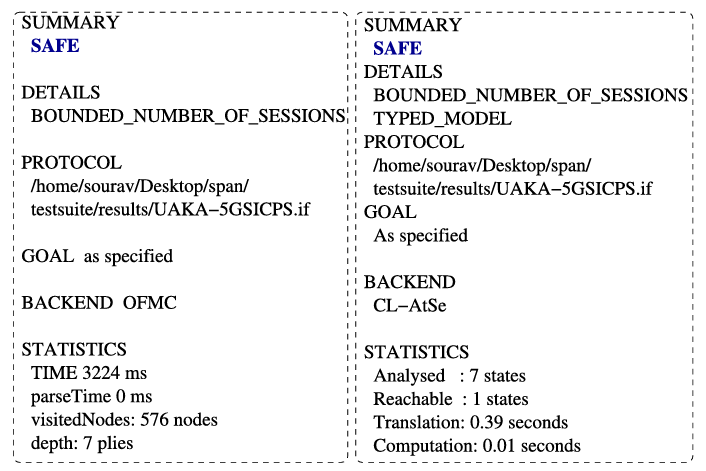
\includegraphics[width=0.8\linewidth]{fig6.png} % Adjust the path and filename
        \caption{Simulation results under OFMC and CL-AtSe backends.}
        \label{fig:simulation_results}
    \end{figure}
\end{frame}

\section{MIRACL}
\begin{frame}
    \frametitle{VI. Experiment Setup for MIRACL}
    \begin{itemize}
        \item \textbf{Cryptographic Library Used:} 
            \begin{itemize}
                \item Multiprecision Integer and Rational Arithmetic Cryptographic Library (MIRACL) \cite{miracl2020}.
            \end{itemize}
        \item \textbf{Platforms:}
            \begin{itemize}
                \item \textbf{Server Environment:}
                    \begin{itemize}
                        \item Model: MacBook Pro (2019)
                        \item CPU Architecture: 64-bit
                        \item Processor: 2.3 GHz Intel Core i9
                        \item Memory: 32 GB
                        \item OS: macOS Mojave 10.14.6
                    \end{itemize}
                \item \textbf{Smart Device Environment:}
                    \begin{itemize}
                        \item Model: Raspberry Pi 3 B+ Rev 1.3
                        \item CPU: 64-bit, 1.4 GHz Quad-core
                        \item Memory: 1 GB
                        \item OS: Ubuntu 20.04 LTS, 64-bit
                    \end{itemize}
            \end{itemize}
    \end{itemize}
\end{frame}
\begin{frame}
    \frametitle{Measurement of Execution Time}
    \begin{itemize}
        \item \textbf{Cryptographic Primitives:}
            \begin{itemize}
                \item \( T_{ecm} \): Elliptic curve point multiplication
                \item \( T_{eca} \): Elliptic curve point addition
                \item \( T_{h} \): One-way hash function (SHA-256)
                \item \( T_{e} \): Modular exponentiation
                \item \( T_{bp} \): Bilinear pairing operation
                \item \( T_{senc} \): Symmetric encryption
                \item \( T_{sdec} \): Symmetric decryption
                \item \( T_{ibe\text{-}keygen} \): Key generation for ID-based encryption
                \item \( T_{ibe\text{-}enc} \): ID-based encryption
                \item \( T_{ibe\text{-}dec} \): ID-based decryption
            \end{itemize}
        \item \textbf{Methodology:}
            \begin{itemize}
                \item Each cryptographic primitive executed for 100 runs.
                \item Average run-time measured in milliseconds.
            \end{itemize}
    \end{itemize}
\end{frame}

\begin{frame}
    \frametitle{Various Cryptographic Primitives Execution Time}
    \begin{figure}
        \centering
        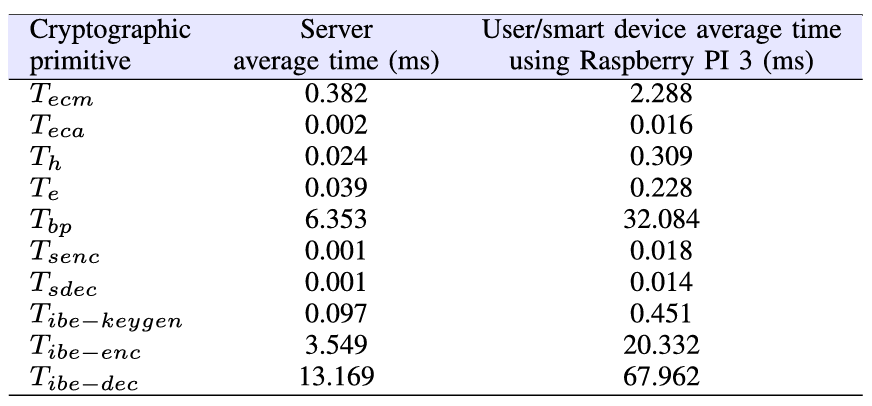
\includegraphics[width=0.9\textwidth]{tabl2.png} % Adjust the path as necessary
        \caption{Execution time of various cryptographic primitives using MIRACL}
    \end{figure}
\end{frame}
\section{Comaparitive Analysis}
\begin{frame}
    \frametitle{VII. Comparative Analysis}
    \begin{itemize}
        \item This section presents a comparative study of the proposed UAKA-5GSICPS scheme against existing competing schemes:
        \begin{itemize}
            \item Harishma et al. [12]%\cite{harishma2018}
            \item Chen et al. [13]%\cite{chen2017}
            \item Chen et al. \cite{chen2019}
        \end{itemize}
        \item We focus on:
        \begin{itemize}
            \item Security and functionality features
            \item Computational costs
            \item Communication costs
        \end{itemize}
        \item The analysis demonstrates the superiority of UAKA-5GSICPS in various aspects compared to the existing schemes.
    \end{itemize}
\end{frame}

\begin{frame}
    \frametitle{1. Security and Functionality Features Comparison}
    \begin{itemize}
        \item Table in the next slide compares essential security and functionality features (F1–F14) among UAKA-5GSICPS and competing schemes.
        \item Key Observations:
        \begin{itemize}
            \item UAKA-5GSICPS demonstrates superior performance across all essential features.
            \item Features include:
            \begin{itemize}
                \item Anonymity and untraceability
                \item Resistance to replay and MiTM attacks
                \item Robust key agreement protocols
            \end{itemize}
        \end{itemize}
        \item Conclusion:
        \begin{itemize}
            \item The comprehensive security functionalities provided by UAKA-5GSICPS position it as a leading solution in the context of ICPS environments.
        \end{itemize}
    \end{itemize}
\end{frame}

\begin{frame}
    \frametitle{Security and Functionality Features Comparison}
    \begin{figure}
        \centering
        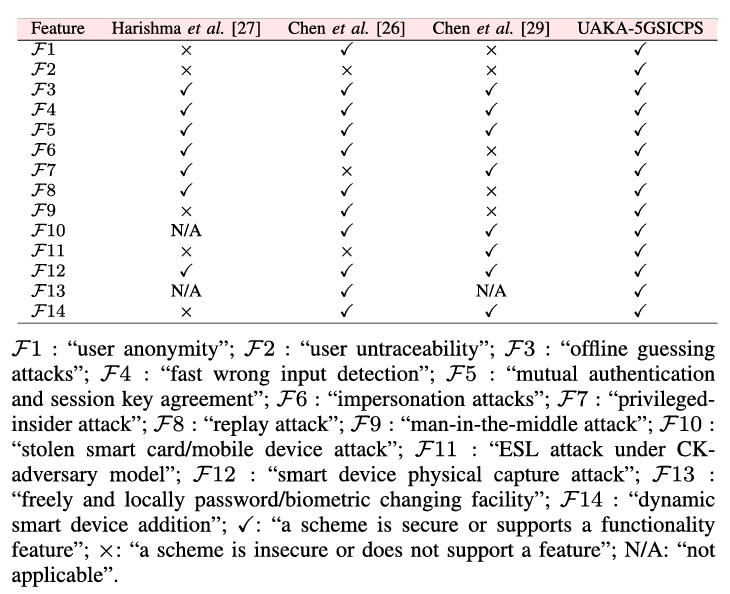
\includegraphics[width=0.9\linewidth]{tabl4.png} % Replace with the path to your image
        \caption{Comparison of security and functionality features among different schemes.}
    \end{figure}
\end{frame}

\begin{frame}
    \frametitle{2. Computational Costs Comparison}
    \begin{itemize}
        \item Focus on the computational costs during the login and authentication key agreement phases.
        \item Costs for UAKA-5GSICPS:
        \begin{itemize}
            \item User \( U_k \): \( T_{fe} + 16 T_h + 5 T_{ecm} + 2 T_{eca} \)
            \item Controller Node \( C_{Ni} \): \( 9 T_h + 3 T_{ecm} + 2 T_{eca} \)
            \item Smart Device \( SD_j \): \( 8 T_h + 4 T_{ecm} + T_{eca} \)
        \end{itemize}
        \item Comparisons:
        \begin{itemize}
            \item UAKA-5GSICPS is comparable to Chen et al. [12] and outperforms Harishma et al. [13] in terms of controller node/server overhead.
            \item Slightly higher overhead on users’ mobile devices, but remains within acceptable limits.
        \end{itemize}
        \item Conclusion:
        \begin{itemize}
            \item The security functionalities offered by UAKA-5GSICPS justify the computational costs incurred.
        \end{itemize}
    \end{itemize}
\end{frame}
\begin{frame}
    \frametitle{3. Communication Costs Comparison}
    \begin{itemize}
        \item Communication cost analysis based on bit-sizes for various components:
        \begin{itemize}
            \item Identity: 160 bits
            \item Random nonce (secret): 160 bits
            \item Current timestamp: 32 bits
            \item Hash output (SHA-1): 160 bits
            \item Elliptic curve point: 320 bits
        \end{itemize}
        \item Transmission Requirements:
        \begin{itemize}
            \item User \( U_k \): 1152 bits
            \item Controller Node \( C_{Ni} \): 1024 bits
            \item Smart Device \( SD_j \): 1024 bits
        \end{itemize}
        \item Total Communication Cost: 3200 bits for three messages.
        \item Comparison with Competing Schemes:
        \begin{itemize}
            \item UAKA-5GSICPS is comparable to Chen et al. [12]
 and Chen et al. \cite{chen2019}.
            \item Outperforms Harishma et al. [13]
 in communication efficiency.
        \end{itemize}
        \item Conclusion:
        \begin{itemize}
            \item UAKA-5GSICPS balances security and efficiency in communication costs.
        \end{itemize}
    \end{itemize}
\end{frame}
\begin{frame}
    \frametitle{Comparison Tables}
    \begin{figure}
        \centering
        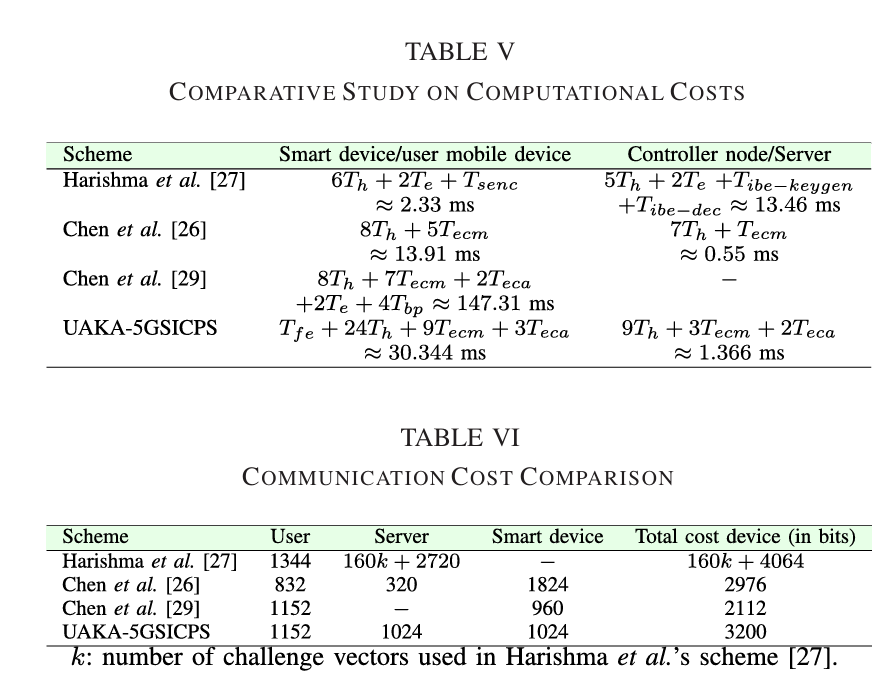
\includegraphics[width=0.9\linewidth]{comptable.png} % Replace with the path to your image
        \caption{Comparative Study on Computational Costs and Computational Costs Comparison}
    \end{figure}
\end{frame}

\begin{frame}
    \frametitle{Concluding Remarks (Part 1)}
    \begin{itemize}
        \item \textbf{Overview of the Study:}
        \begin{itemize}
            \item Discussed security aspects of SDN-based ICPS environments.
            \item Designed a novel secure user authentication and key agreement scheme (UAKA-5GSICPS).
        \end{itemize}
        \item \textbf{Key Features of UAKA-5GSICPS:}
        \begin{itemize}
            \item \textbf{Three-factor authentication:} 
            \begin{itemize}
                \item User password
                \item Mobile device
                \item Personal biometrics
            \end{itemize}
            \item Supports mutual authentication and session key establishment.
            \item Allows dynamic addition of smart devices and user credential changes without RA communication.
        \end{itemize}
    \end{itemize}
\end{frame}
\begin{frame}
    \frametitle{Concluding Remarks (Part 2)}
    \begin{itemize}
        \item \textbf{Security Analysis:}
        \begin{itemize}
            \item Formal and informal analyses demonstrate resilience against modern attacks.
            \item AVISPA tool verification confirms security against replay and MiTM attacks.
            \item Offers functionalities such as user anonymity and traceability.
        \end{itemize}
        \item \textbf{Comparative Analysis:}
        \begin{itemize}
            \item UAKA-5GSICPS is comparable in computational and communication costs to other schemes.
            \item Feasible for practical applications, including medical CPS and vehicular transportation.
        \end{itemize}
        \item \textbf{Future Work:}
        \begin{itemize}
            \item Explore secure user authentication and session key establishment in SDNs with distributed control plane architecture.
        \end{itemize}
    \end{itemize}
\end{frame}

\section*{References}

\bibliographystyle{IEEEtran}
\bibliography{references}

\end{document}
